\chapter*{第三部分:突触传递}
\markboth{突触传递}{突触传递}


\begin{figure}[htbp]
	\centering
	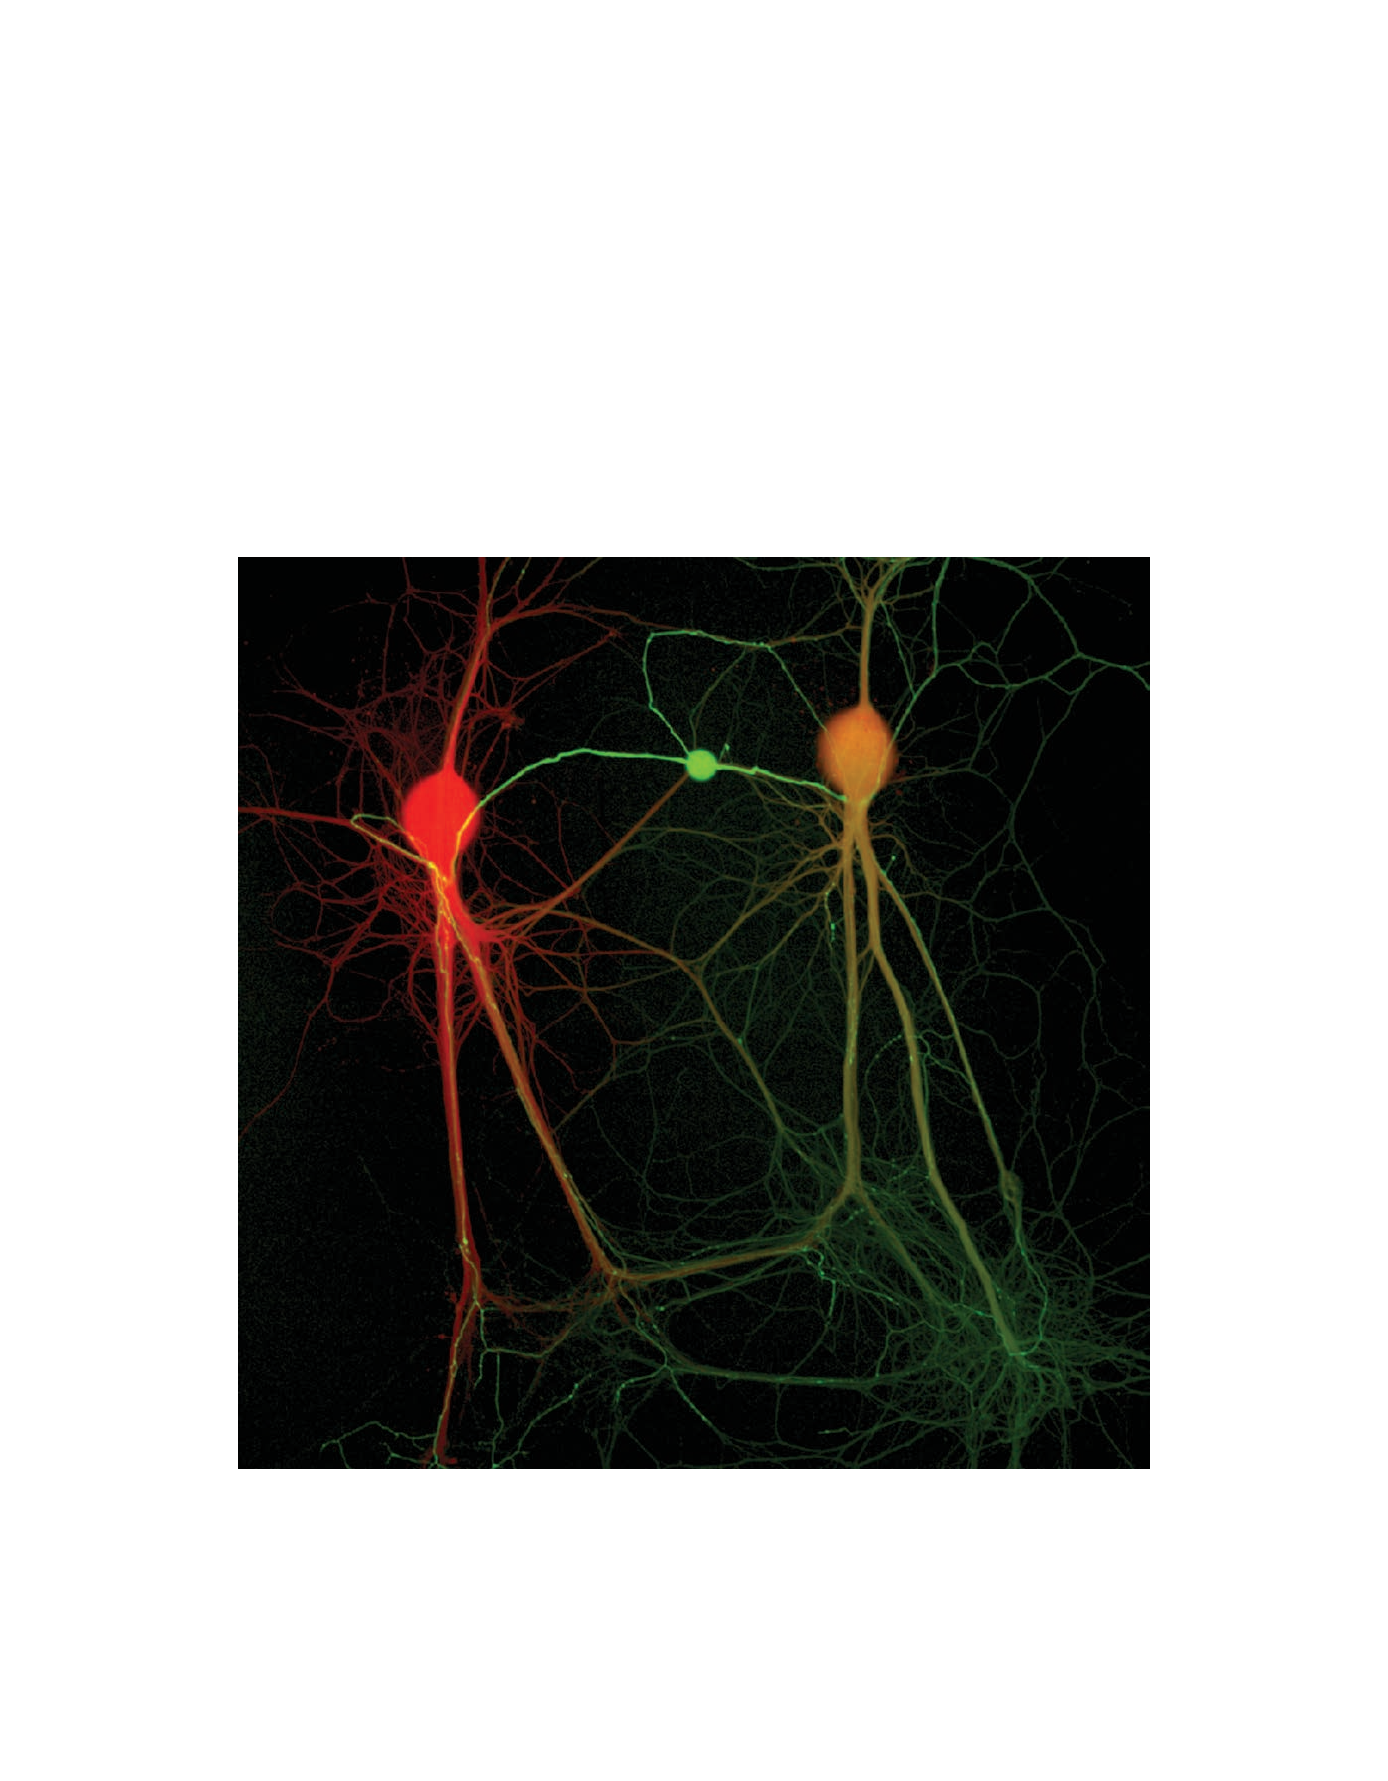
\includegraphics[width=0.9\linewidth]{chap11/fig_11_0}
	\caption{在细胞培养中,机械感觉神经元(中心,绿色)发送其轴突与两个运动神经元(红色,橙色)形成兴奋性突触连接,概括了活体动物中的连接。
		这些神经元是从加利福尼亚海螺中分离出来的。}
	\label{fig:11_0}
\end{figure}


在第二部分中,我们研究了电信号是如何在单个神经元内启动和传播的。
我们现在转向突触传递,即一个神经细胞与另一个细胞交流的过程。


除了一些例外,突触由三个组成部分组成:
(1)突触前轴突的末端,
(2)突触后细胞上的靶标,以及(3)并置区。
根据并置的结构,突触分为两大类:
电突触和化学突触。
在电突触中,突触前末端和突触后细胞在称为间隙连接的区域非常紧密地并置。
突触前神经元中动作电位产生的电流通过称为间隙连接通道的特殊桥接通道直接进入突触后细胞,间隙连接通道物理连接突触前和突触后细胞的细胞质。
在化学突触上,两个细胞之间有一道裂缝,细胞不能通过桥接通道进行交流。
相反,突触前细胞的动作电位会导致神经末梢释放化学递质。
递质在突触间隙扩散,并与突触后膜上的受体分子结合,后者调节突触后细胞中离子通道的打开和关闭。
这导致突触后神经元的膜电位发生变化,该神经元可以刺激或抑制动作电位的释放。


神经递质的受体可分为两大类,这取决于它们如何控制突触后细胞中的离子通道。
一种类型是离子型受体,它是一种在发射器结合时打开的离子通道。
第二种类型,代谢型受体,通过激活突触后细胞内的生化第二信使级联,间接作用于离子通道。
这两种类型的受体都可以导致兴奋或抑制。
信号的符号不取决于发射器的身份,而是取决于发射器与之相互作用的受体的性质。
大多数递质都是低分子量分子,但某些肽也可以作为突触的信使。
电生理学、生物化学和分子生物学的方法已被用于表征突触后细胞中对这些不同化学信使作出反应的受体。
这些方法还阐明了第二信使通路如何在细胞内转导信号。


在本书的这一部分,我们认为突触传递是最基本的形式。
我们首先比较和对比两大类突触,\textit{化学突触}和\textit{电突触}(见第~\ref{chap:chap11}~章)。
然后,我们将重点放在外周神经系统中的化学突触模型上,即突触前运动神经元和突触后骨骼肌纤维之间的\textit{神经肌肉接头}(见第~\ref{chap:chap12}~章)。
接下来,我们研究中枢神经系统神经元之间的\textit{化学突触},重点是突触后细胞及其对来自多个突触前输入的突触信号的整合,这些信号同时作用于\textit{离子型受体}(见第~\ref{chap:chap13}~章)和\textit{代谢型受体}(参见第~\ref{chap:chap14}~章)。
然后,我们转向突触前末梢,考虑神经元从突触前末端释放递质的机制,神经活动如何调节\textit{递质的释放}(见第~\ref{chap:chap15}~章),以及神经递质的\textit{化学性质}(见第~\ref{chap:chap16}~章)。
由于化学突触的分子结构是复杂的,许多遗传性疾病和获得性疾病都会影响化学突触的传递,我们将在稍后的第~\ref{chap:chap57}~章进行详细讨论。


贯穿本节各章以及整本书的一个关键主题是\textit{可塑性}的概念。
在所有突触中,突触连接的强度不是固定的,而是可以通过行为背景或经验,通过被称为突触可塑性的各种机制,以各种方式进行改变。
一些修饰是由突触本身的活动引起的(\textit{同突触可塑性})。
其他修饰取决于外在因素,通常是由于调节递质的释放(\textit{异突触可塑性})。
在第~\ref{chap:chap53}~章和第~\ref{chap:chap54}~章中,我们将看到这种修改如何为不同形式的记忆存储提供\textit{细胞基质},其持续时间从几秒钟到一生。
在第九部分的章节中,我们将看到突触可塑性功能障碍如何导致各种神经疾病和精神疾病。



\chapter{突触传递概述} \label{chap:chap11}

是什么赋予神经细胞以如此精确且快速相互交流的特殊能力?
我们已经看到信号是如何在神经元\textit{内}传播的,从它的树突和细胞体到它的轴突末端。
在本章中,我们开始考虑神经元\textit{之间}通过突触传递过程发出的信号。
突触传递是我们在本书中讨论的神经功能的基础,例如感知、自主运动和学习。


神经元在称为突触的专门部位相互交流。
平均每个神经元形成数千个突触连接并接收相似数量的输入。
然而,这个数字可能会因神经元的特定类型而有很大差异。
小脑的\textit{浦肯野细胞}接收多达 10 万个突触输入,而邻近的颗粒神经元(大脑中数量最多的一类神经元)仅接收约四个兴奋性输入。
尽管中枢神经系统和周围神经系统中的许多突触连接是高度专业化的,但所有神经元都利用突触传递的两种基本形式之一:电或化学。
此外,两种形式的突触传递的强度不是固定的,而是可以通过神经元活动增强或减弱。
这种突触可塑性对于记忆和其他高层大脑功能至关重要。


电突触主要用于发送\textit{快速}和\textit{定型}的去极化信号。
相反,化学突触能够发出更多\textit{可变}的信号,因此可以产生更复杂的相互作用。
它们可以在突触后细胞中产生\textit{兴奋}性或\textit{抑制}性作用,并引发突触后细胞持续几毫秒到几小时的变化。
化学突触还可以\textit{放大}神经元信号,因此即使是一个小的突触前神经末梢也可以改变大的突触后细胞的反应。
由于化学突触传递对于理解大脑和行为至关重要,因此将在接下来的四章中对其进行详细研究。



\section{突触主要是电突触或化学突触}

突触一词由\textit{查尔斯$\cdot$谢林顿}在 20 世纪初引入,用于描述一个神经元与另一个神经元通信的专门接触区。
19 世纪后期,\textit{拉蒙-卡哈尔}首次在光学显微镜水平上对该部位进行了组织学描述。


所有的突触最初都被认为是通过电传输来运作的。
然而,在 20 世纪 20  年代,\textit{奥托$\cdot$勒维}发现一种化合物,很可能是\textit{乙酰胆碱},可以从迷走神经传递信号以减慢心跳。
\textit{勒维}的发现在 20世纪 30 年代引发了关于化学信号是否存在于运动神经和骨骼肌之间的快速突触以及大脑突触中的大量争论。


出现了两种思想流派,一种是生理学派,另一种是药理学派。
每一种流派都支持单一的机制用于所有突触传递。
在\textit{约翰$\cdot$埃克尔斯}(\textit{谢林顿}的学生)的带领下,\textit{生理}学家认为突触传递是\textit{电}的,突触前神经元中的动作电位会产生被动流入突触后细胞的电流。
以\textit{亨利$\cdot$戴尔}为首的\textit{药理}学家认为,传递是\textit{化学}的,突触前神经元中的动作电位会导致化学物质的释放,而化学物质又会在突触后细胞中启动电流。
当生理学和超微结构技术在 20 世纪50 年代和 60 年代得到改进时,很明显两种传播形式都存在。
虽然大多数神经元通过化学递质启动电信号,但许多其他神经元直接在突触后细胞中产生电信号。


一旦用电子显微镜可以看到突触的精细结构,就会发现化学突触和电突触具有不同的结构。
在化学突触中,突触前和突触后神经元被一个小空间完全分开,即突触间隙;
一个细胞和下一个细胞的细胞质之间没有连续性。
相反,在电突触处,突触前和突触后细胞通过直接连接两个细胞细胞质的特殊通道进行通信。


表~\ref{tab:11_1}~总结了两种突触的主要功能特性。
通过将正电流注入突触前细胞以引发去极化,可以观察到最重要的差异。
在这两种类型的突触中,穿过突触前细胞膜的外向电流在其膜内部沉积正电荷,从而使细胞去极化(第~\ref{chap:chap9}~章)。
在电突触处,一些电流将通过\textit{间隙连接通道}进入突触后细胞,在膜内部沉积正电荷并使其去极化。
电流通过静息通道跨膜离开突触后细胞(图~\ref{fig:11_1}A)。
如果去极化超过阈值,突触后细胞中的电压门控离子通道会打开并产生动作电位。
相比之下,在化学突触处,突触前细胞和突触后细胞之间没有直接的低电阻通路。
相反,突触前神经元中的动作电位启动化学递质的释放,化学递质扩散穿过\textit{突触间隙}并与突触后细胞膜上的受体结合(图~\ref{fig:11_1}B)。


\begin{table}[htbp]
	\caption{电突触和化学突触的区别性质} \label{tab:11_1} \centering
	\begin{tabular}{lllllll}
		\toprule
		突触类型 & \makecell{突触前和\\突触后细胞膜\\之间的距离} & \makecell{突触前和\\突触后细胞之间\\的细胞质连续性} & 超微结构成分 & 传输代理 & 突触延迟 & 传输方向 \\
		\midrule
		电 & 4 纳米 & 是 & 间隙连接通道 & 离子电流 & 几乎没有 & 通常是双向 \\
		化学 & 20-40 纳米 & 否 & \makecell[l]{突触前小泡\\和活动区;\\突触后受体} & 化学递质 & \makecell[l]{显著:至\\少0.3毫秒,\\通常为1-5毫秒\\或更长时间} & 单向 \\
		\bottomrule
	\end{tabular}
\end{table}


\begin{figure}[htbp]
	\centering
	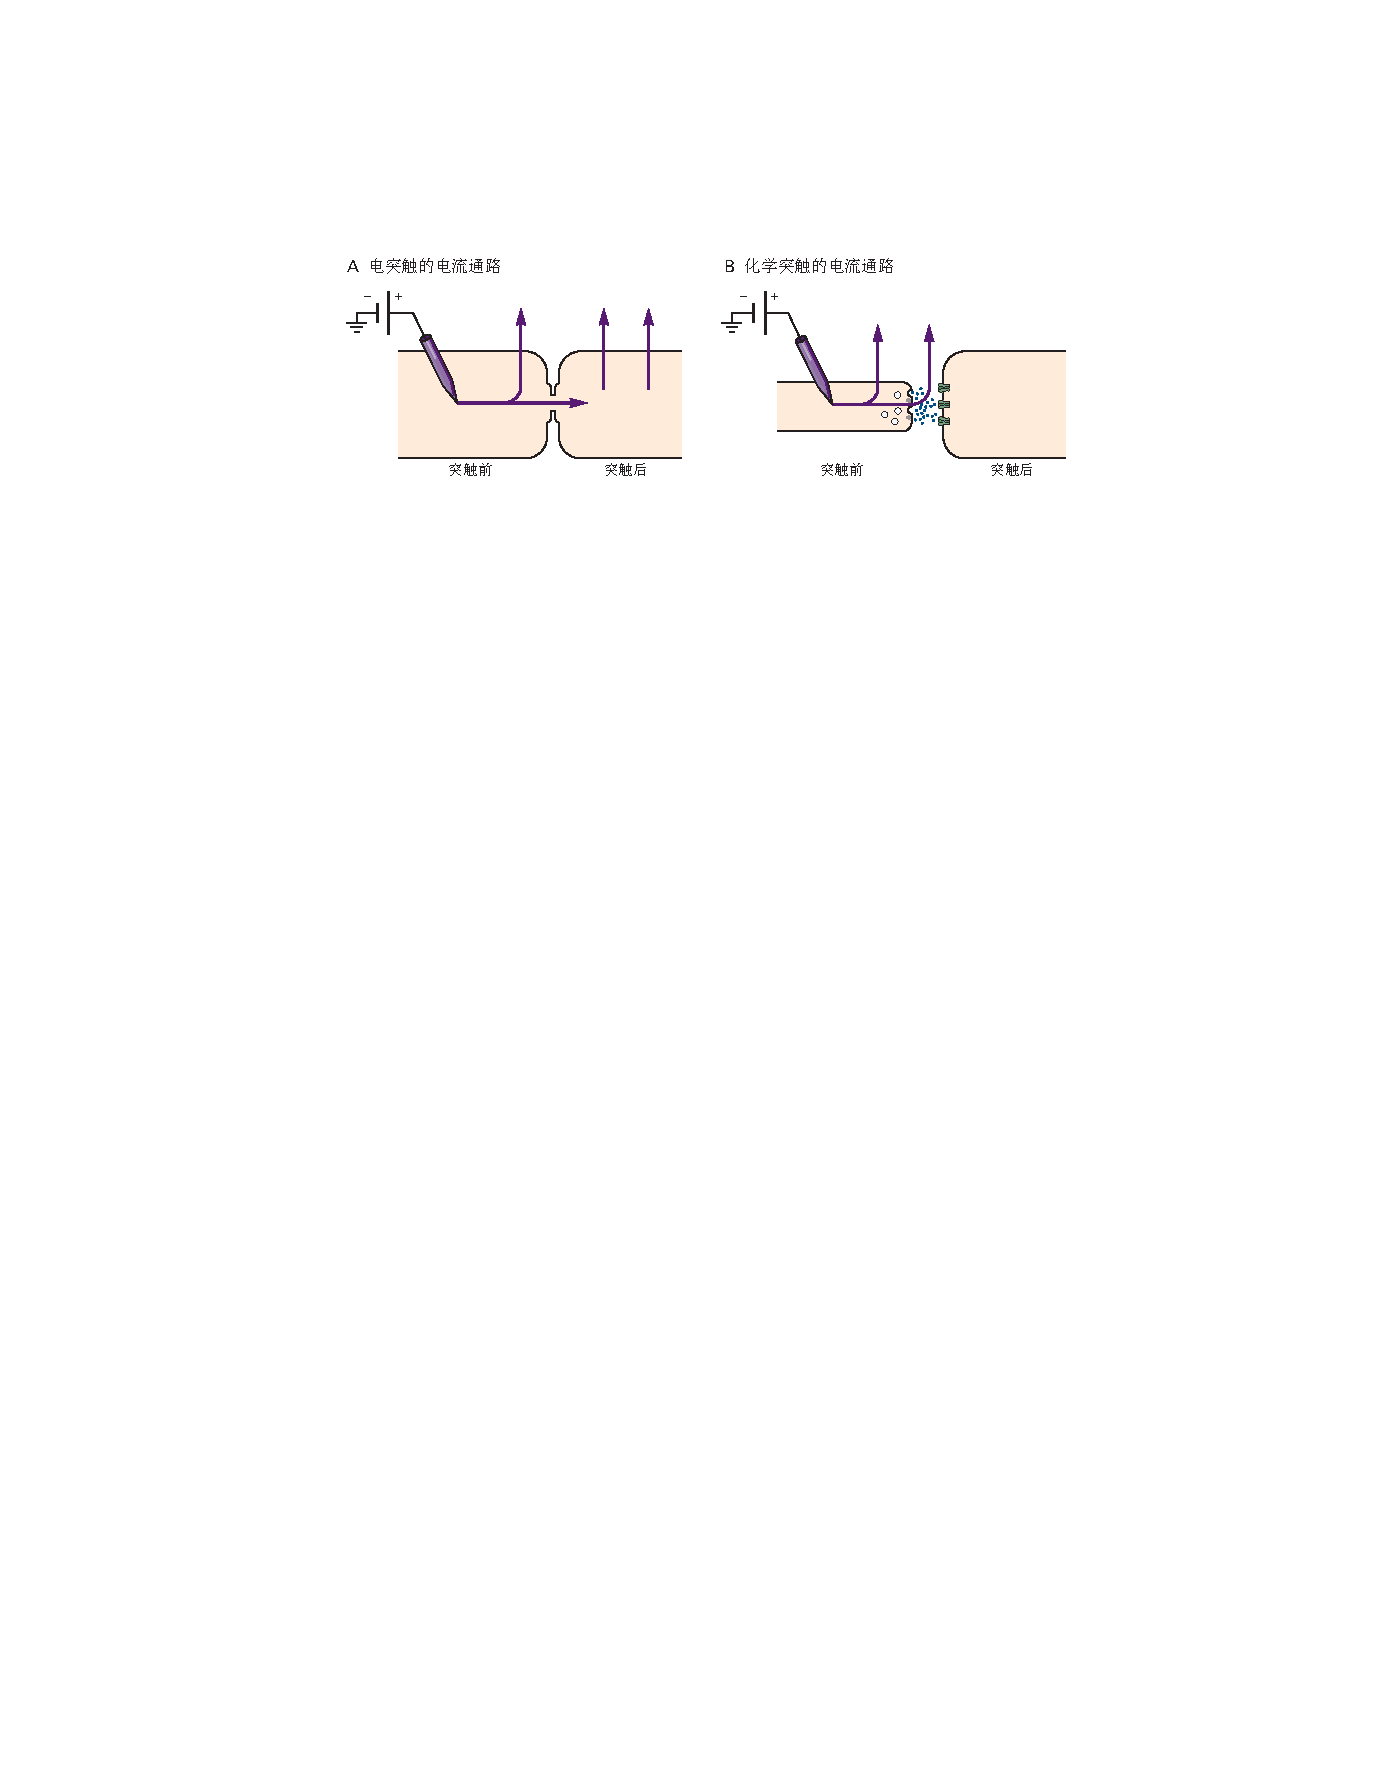
\includegraphics[width=0.85\linewidth]{chap11/fig_11_1}
	\caption{电突触和化学突触的功能特性。
		\textbf{A.} 在\textit{电突触}处,一些注入\textit{突触前}细胞的电流通过细胞膜中的静息(非门控)离子通道逸出。
		然而,一些电流也通过间隙连接通道进入\textit{突触后}细胞,间隙连接通道连接突触前细胞和突触后细胞的细胞质,并为电流提供低电阻(高电导)通路。
		\textbf{B.} 在\textit{化学突触}处,所有注入突触前细胞的电流都会逃逸到细胞外液中。
		然而,由此产生的突触前细胞膜去极化会产生动作电位,导致释放与\textit{突触后}细胞上的受体结合的神经递质分子。
		这种结合打开离子通道,引发突触后细胞膜电位的变化。}
	\label{fig:11_1}
\end{figure}


\section{电突触提供快速信号传输}

在电突触的兴奋性突触传递过程中,突触前细胞中的电压门控离子通道产生使突触后细胞去极化的电流。
因此,这些通道不仅使突触前细胞在动作电位阈值以上去极化,而且产生足够的离子电流以在突触后细胞中产生电位变化。
要产生如此大的电流,突触前末端必须足够大,以使其膜包含许多离子通道。
同时,突触后细胞必须相对较小。
这是因为小细胞比大细胞具有更高的输入电阻($R_{in}$),并且根据欧姆定律($\Delta V = I \times R_{in}$),响应给定的突触前电流($I$),会经历更大的电压变化($\Delta V$)。


电突触传递首先由\textit{爱德华$\cdot$弗斯潘}和\textit{大卫$\cdot$波特}在小龙虾的巨大运动突触中描述,其中突触前纤维比突触后纤维大得多(图~\ref{fig:11_2}A)。
突触前纤维中产生的动作电位会产生去极化的突触后电位,该电位通常超过激发动作电位的阈值。
在电突触处,突触延迟(突触前尖峰和突触后电位之间的时间)非常短(图~\ref{fig:11_2}B)。


\begin{figure}[htbp]
	\centering
	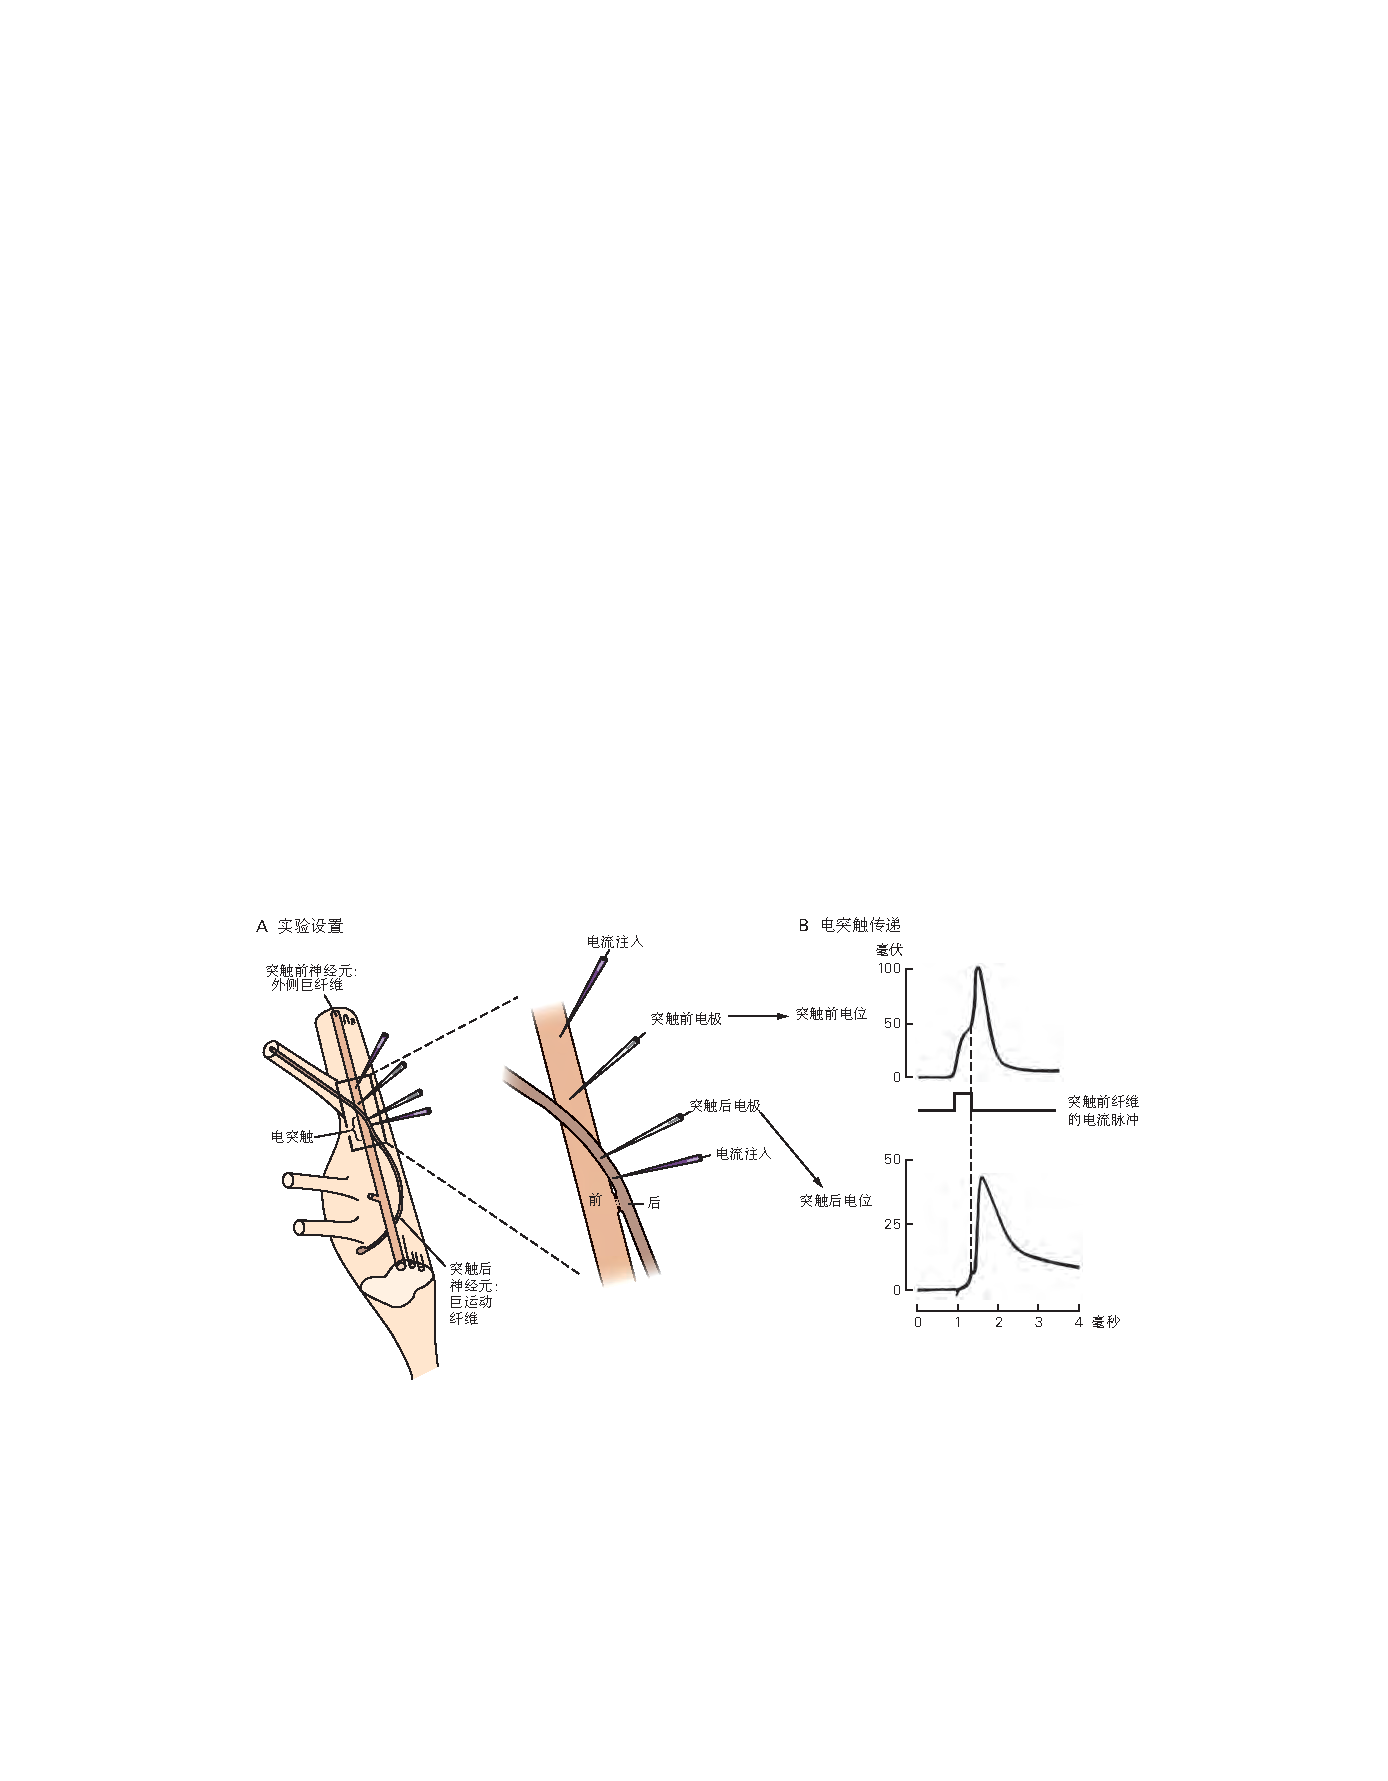
\includegraphics[width=1.0\linewidth]{chap11/fig_11_2}
	\caption{电突触传递首先在小龙虾的巨大运动突触中得到证实\cite{furshpan1959transmission,furshpan1957mechanism}。 
		\textbf{A.} 沿着神经索向下延伸的横向巨大纤维是突触前神经元。
		从神经节内的细胞体向周围突出的巨型运动纤维就是突触后神经元。
		用于传递电流和记录电压的电极放置在突触前和突触后细胞内。
		\textbf{B.} 电突触的传输实际上是瞬时的,即突触后反应在几分之一毫秒内跟随突触前刺激。
		虚线显示了两个细胞的响应如何及时对应。
		在化学突触处,突触前电位和突触后电位之间存在延迟(突触延迟)(见图~\ref{fig:11_8})。}
	\label{fig:11_2}
\end{figure}


\begin{figure}[htbp]
	\centering
	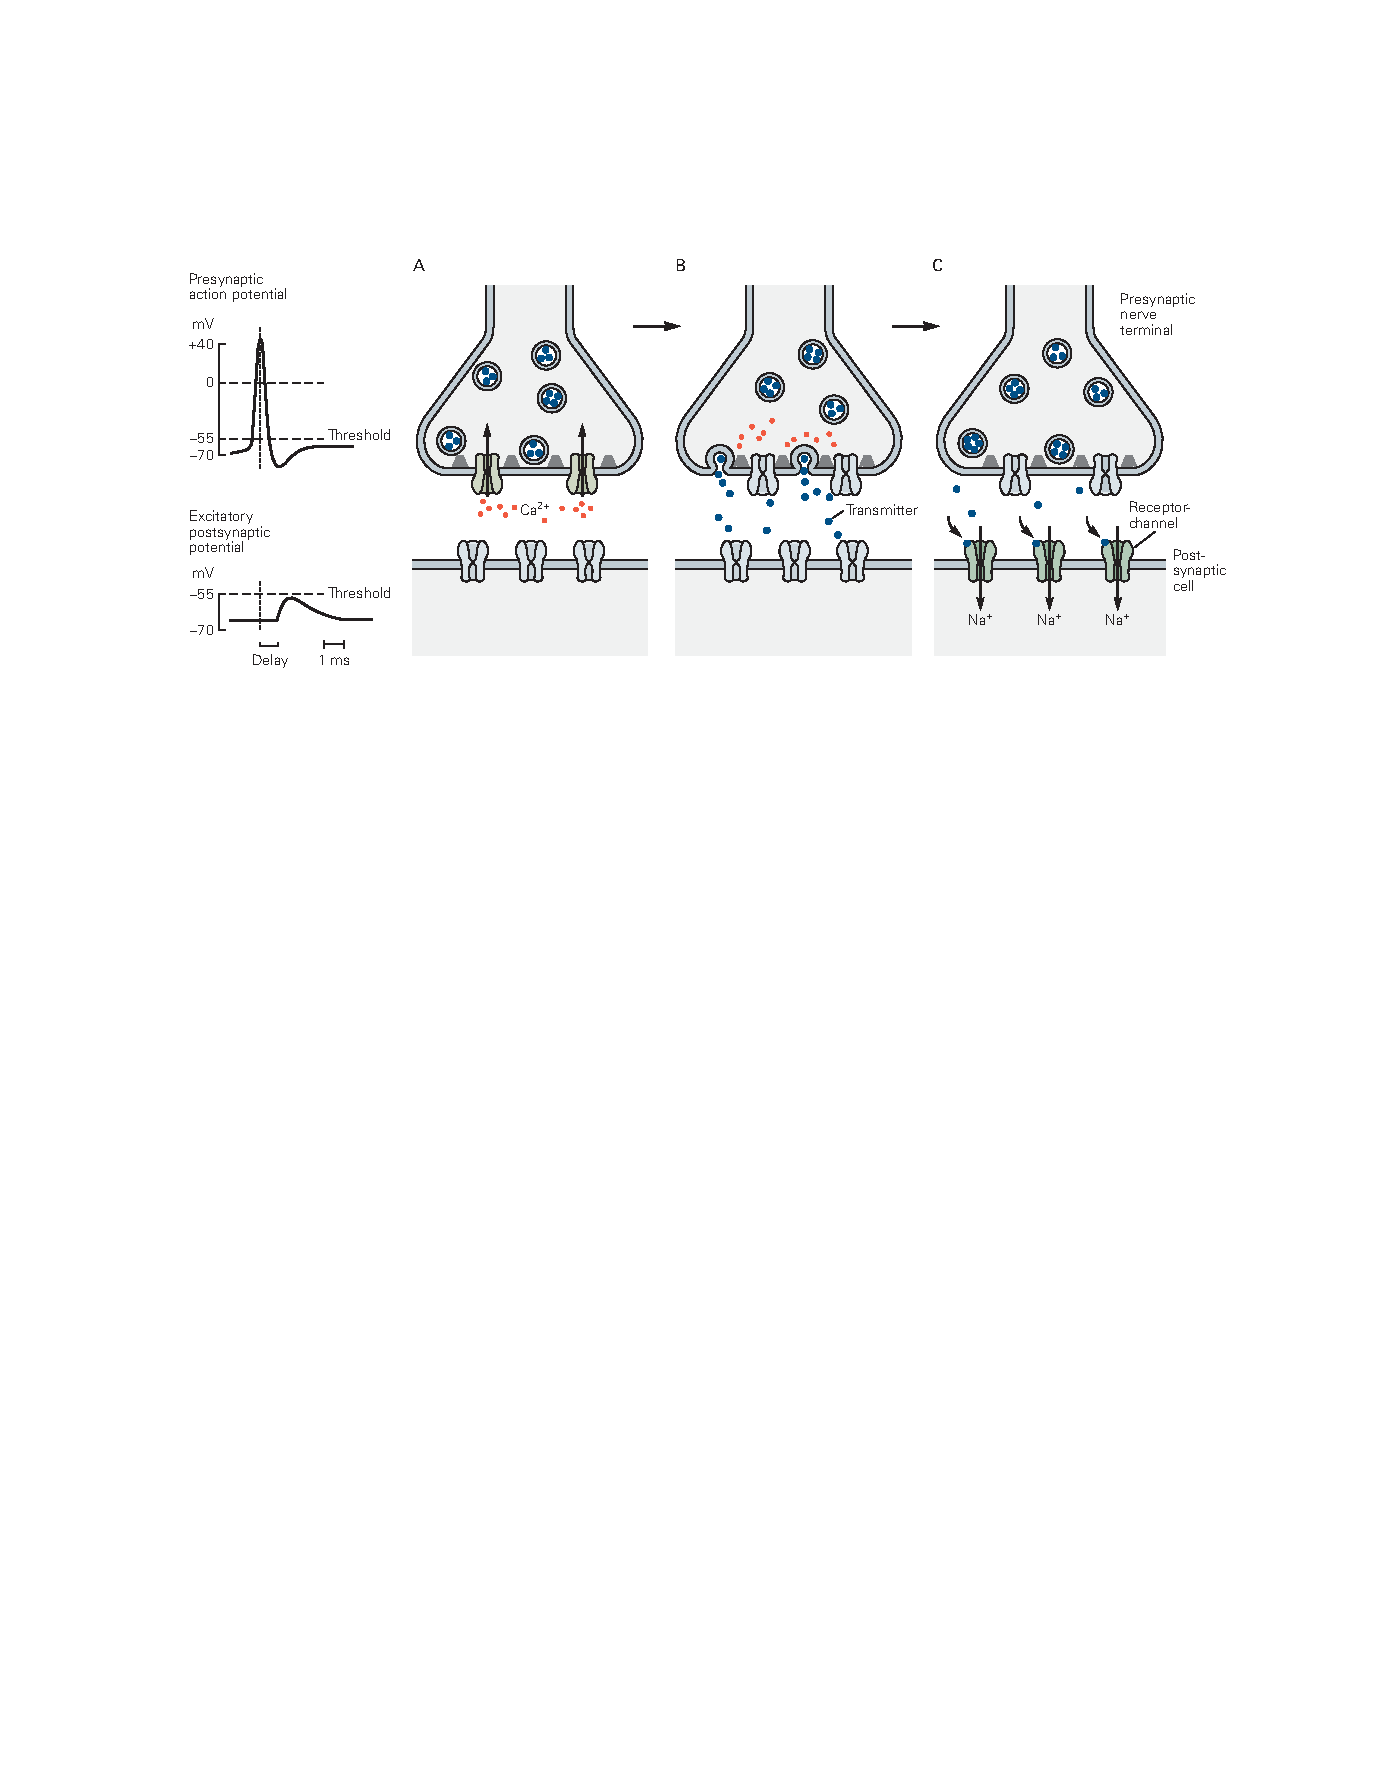
\includegraphics[width=1.0\linewidth]{chap11/fig_11_8}
	\caption{化学突触的突触传递涉及几个步骤。
		化学突触传递的复杂过程解释了突触前细胞中的动作电位与突触后细胞中的突触电位之间的延迟,与电突触处几乎瞬时的信号传递相比(见图~\ref{fig:11_2}B)。
		\textbf{A.} 到达突触前轴突末端的动作电位导致活动区的电压门控 \ce{Ca^2+} 通道打开。
		灰色细丝代表活性区的对接和释放位点。
		\textbf{B.} 钙离子通道开放在活性区附近产生高浓度的细胞内钙离子,导致含有神经递质的囊泡与突触前细胞膜融合并将其内容物释放到突触间隙(称为胞吐作用的过程)。
		\textbf{C.} 释放的神经递质分子然后扩散到突触间隙并结合突触后膜上的特定受体。
		这些受体导致离子通道打开(或关闭),从而改变突触后细胞的膜电导和膜电位。}
	\label{fig:11_8}
\end{figure}


化学传递不可能出现如此短的潜伏期,这需要几个生化步骤:
从突触前神经元释放递质,递质分子穿过突触间隙扩散到突触后细胞,递质与特定受体的结合,以及随后的门控 离子通道(本章和下一章均有描述)。
只有电流直接从一个细胞流向另一个细胞才能产生在巨电机电突触处观察到的近乎瞬时的传输。


电传输的另一个特点是突触后细胞电位的变化与突触前细胞电位变化的大小和形状直接相关。
即使将微弱的亚阈值去极化电流注入突触前神经元,一些电流也会进入突触后细胞并使其去极化(图~\ref{fig:11_3})。
相反,在化学突触中,突触前细胞中的电流必须达到动作电位的阈值,然后才能释放递质并在突触后细胞中引起反应。


\begin{figure}[htbp]
	\centering
	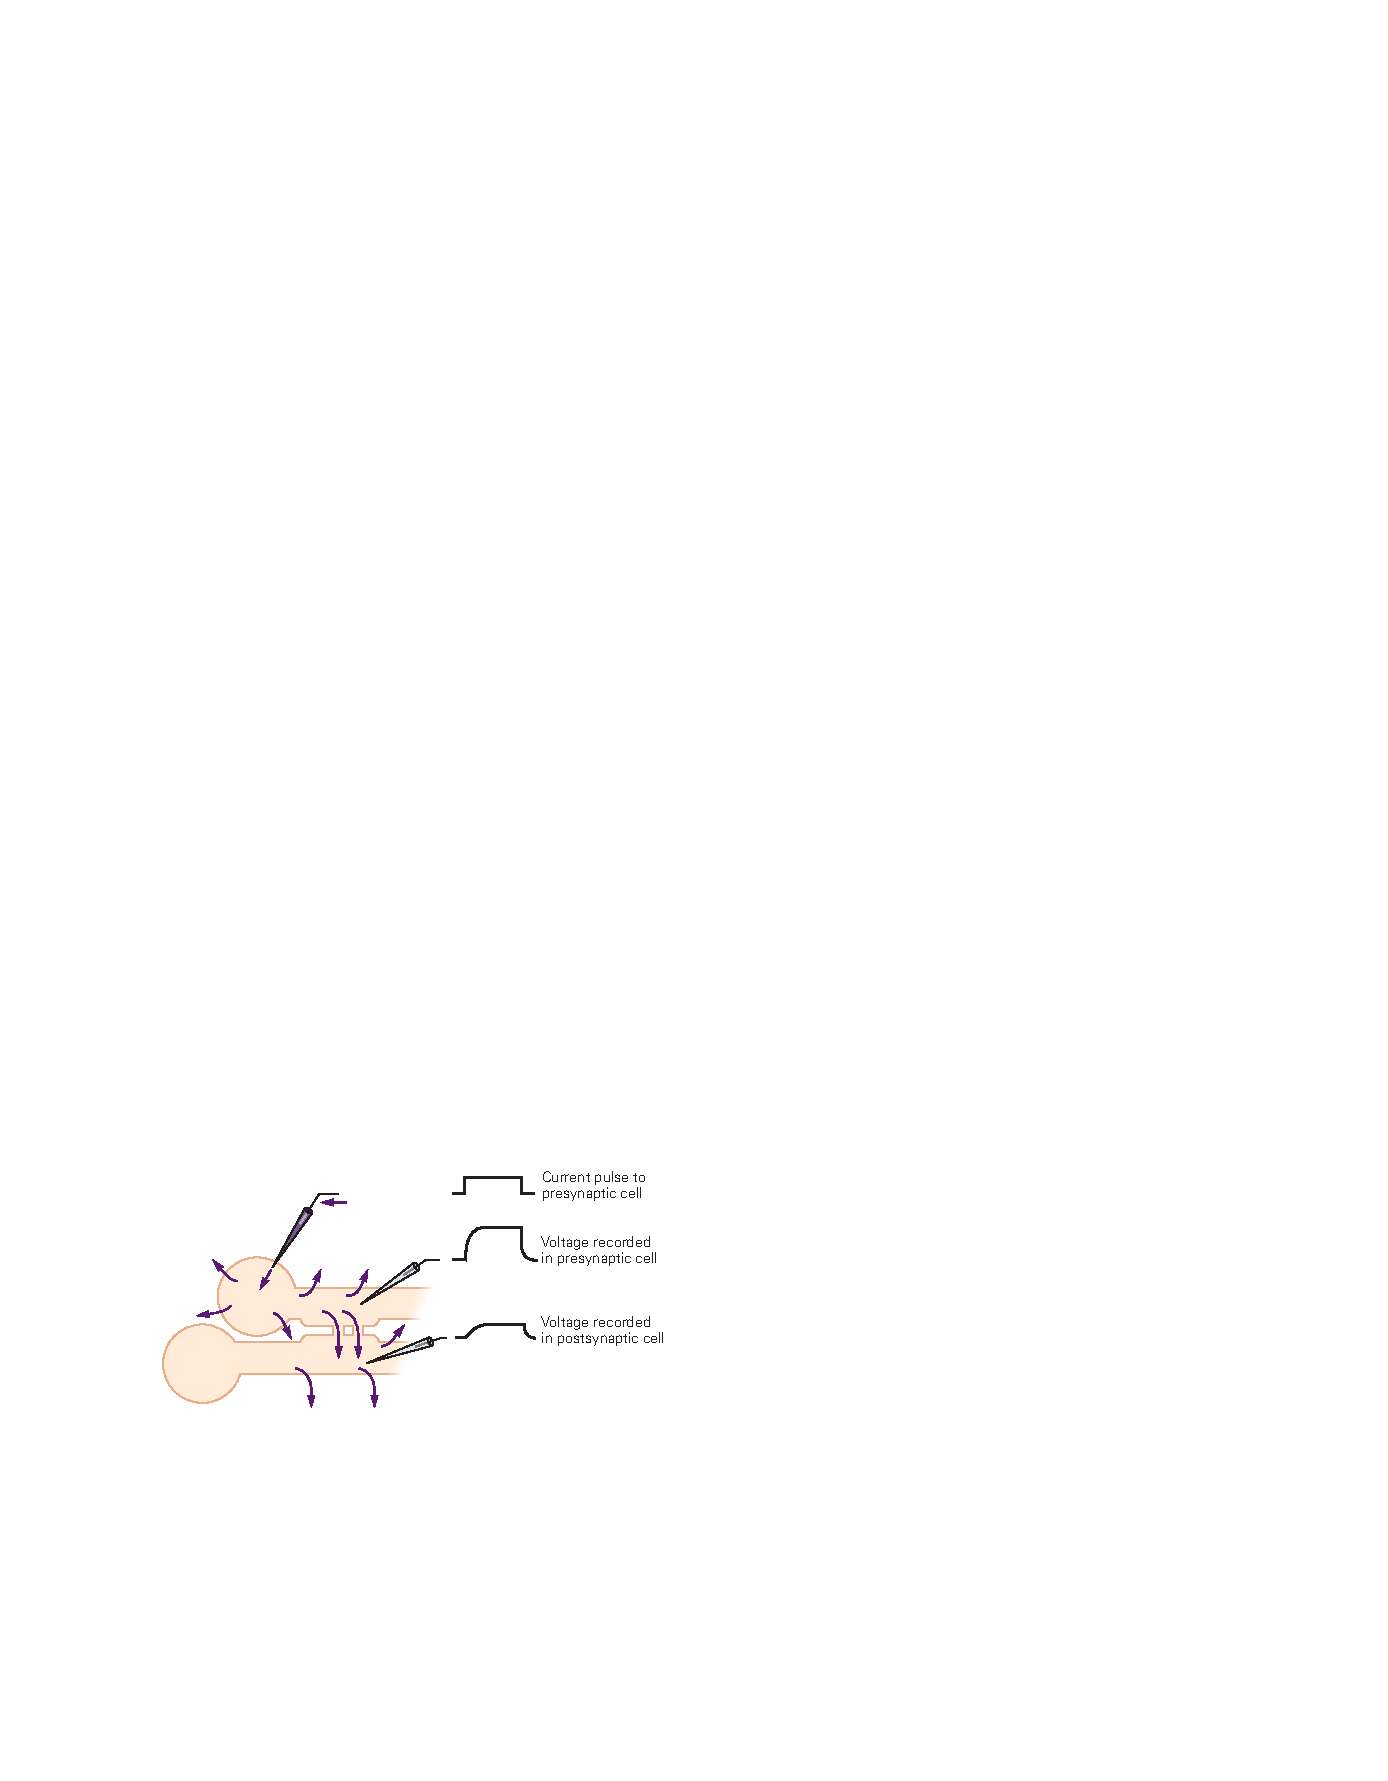
\includegraphics[width=0.6\linewidth]{chap11/fig_11_3}
	\caption{电传输是分级的。
		即使突触前细胞中的电流低于动作电位的阈值,它也会发生。
		如单细胞记录所示,亚阈值去极化刺激会导致突触前和突触后细胞发生被动去极化。
		(去极化或外向电流由向上偏转表示。)}
	\label{fig:11_3}
\end{figure}


大多数电突触可以传输去极化和超极化电流。
具有较大超极化后电位的突触前动作电位会在突触后细胞中产生双相(去极化-超极化)电位变化。
电突触处的信号传输类似于亚阈值电信号沿轴突的被动传播(第~\ref{chap:chap9}~章),因此也称为\textit{电紧张传输}。
在一些专门的间隙连接处,通道具有电压依赖性门控,允许它们仅在一个方向上传导去极化电流,即从突触前细胞到突触后细胞。
这些连接点称为\textit{矫正突触}
(小龙虾的巨型运动突触就是一个例子)。



\subsection{电突触处的细胞通过间隙连接通道连接}

在电突触处,突触前和突触后成分并列在间隙连接处,其中两个神经元之间的间隔(4 纳米)远小于神经元之间的正常非突触间隙(20 纳米)。
这个狭窄的间隙由间隙连接通道桥接,间隙连接通道是一种特殊的蛋白质结构,可将离子电流直接从突触前细胞传导至突触后细胞。


间隙连接通道由一对半通道或连接子组成,一个位于突触前,另一个位于突触后细胞膜。
因此,这些半通道在两个细胞之间形成了一个连续的桥梁(图~\ref{fig:11_4})。
通道的孔具有约 1.5 纳米的大直径,远大于离子选择性配体门控或电压门控通道的 0.3 至 0.5 纳米直径。
间隙连接通道的大孔不区分无机离子,甚至足够宽以允许小有机分子和荧光染料等实验标记物在两个细胞之间通过。


\begin{figure}[htbp]
	\centering
	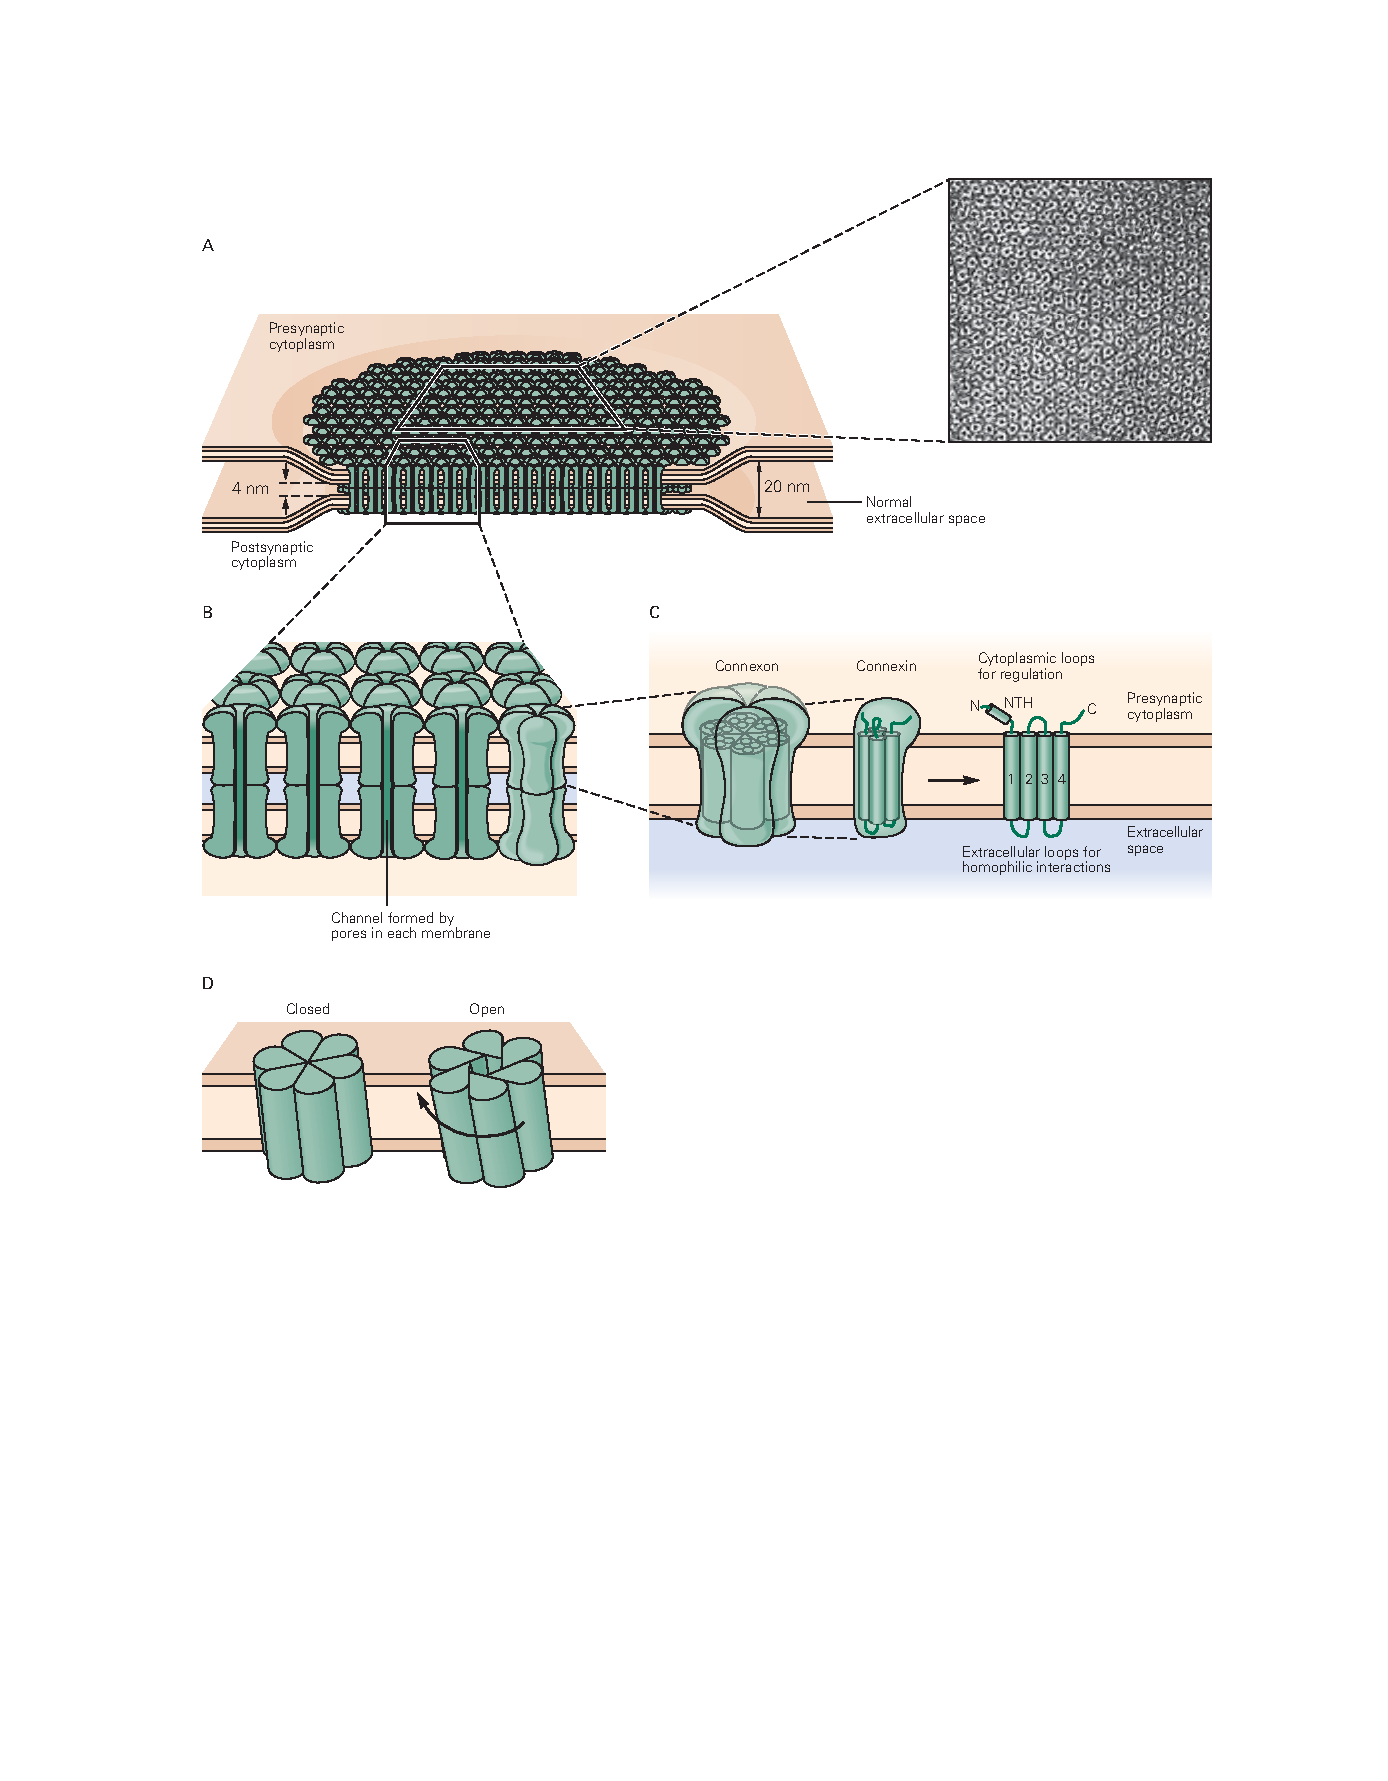
\includegraphics[width=1.0\linewidth]{chap11/fig_11_4}
	\caption{基于 X 射线和电子衍射研究的间隙连接通道的三维模型。
		答:电突触或间隙连接由许多跨越突触前和突触后神经元膜的专门通道组成。
		这些间隙连接通道允许电流直接从一个细胞传递到另一个细胞。
		电子显微照片中的通道阵列是从大鼠肝细胞膜中分离出来的,该细胞膜已被负染色,这种技术使通道周围和毛孔中的区域变暗。
		每个通道的轮廓都是六角形的。
		放大倍率 ×307,800。
		\textbf{B.} 间隙连接通道实际上是一对半通道,每个对应细胞中都有一个连接两个细胞的细胞质\cite{makowski1977gap}。 
		\textbf{C.} 每个半通道或连接子由六个相同的亚基(称为连接蛋白)组成。
		每个连接蛋白长约 7.5 纳米,跨越细胞膜。
		单个连接蛋白具有细胞内 N 端和 C 端,包括短的细胞内 N 端 $\alpha$ 螺旋(NTH)和四个跨膜 $\alpha$ 螺旋(1–4)。
		来自许多不同种类组织的间隙连接蛋白的氨基酸序列具有相似区域,包括跨膜螺旋和细胞外区域,它们参与适当半通道的同嗜性匹配。
		\textbf{D.} 连接蛋白的排列方式是在结构的中心形成一个孔。
		由此产生的连接子,孔径约为 1.5 至 2 纳米,具有特征性的六边形轮廓,如 A 部分的照片所示。
		在一些间隙连接通道中,当亚基在 A 处旋转约 0.9 纳米时,孔被打开 细胞质碱基顺时针方向排列\cite{unwin1980structure}。}
	\label{fig:11_4}
\end{figure}


每个连接子由六个相同的亚基组成,称为连接蛋白。
不同组织中的连接蛋白由一个由 21 个独立但相关的基因组成的大家族编码。
在哺乳动物中,神经元中最常见的连接子是由连接蛋白 36 的产物形成的。
连接蛋白基因根据其一级氨基酸序列以其预测分子量(以千道尔顿为单位)命名。
所有连接蛋白亚基都有一个细胞内 N 端和 C 端,中间有四个跨越细胞膜的 $\alpha$ 螺旋(图~\ref{fig:11_4}C)。


不同细胞类型中的许多间隙连接通道由不同连接蛋白基因的产物形成,因此对控制其打开和关闭的调节因子有不同的反应。
例如,尽管大多数缝隙连接通道会因细胞质 pH 值降低或细胞质钙离子升高而关闭,但不同通道亚型对这些因素的敏感性差异很大。
响应于 pH 和钙离子的间隙连接通道的关闭在受损细胞与健康细胞的解偶联中起着重要作用,因为受损细胞含有升高的钙离子水平和高浓度的质子。
最后,从附近的化学突触释放的神经递质可以通过细胞内代谢反应调节间隙连接通道的开放(第~\ref{chap:chap14}~章)。


由人类连接蛋白 26 亚基形成的间隙连接通道的三维结构已通过 X 射线晶体学确定。
该结构显示了跨膜 $\alpha$ 螺旋如何组装形成通道的中心孔,以及连接跨膜螺旋的细胞外环如何交叉连接两个半通道(图~\ref{fig:11_5})。
孔内衬有促进离子运动的极性残基。
N 端 $\alpha$ 螺旋可作为连接蛋白 26 通道的电压门,在关闭状态下堵塞孔的细胞质口。
从功能研究中推断出通道细胞外侧有一个单独的门,由连接前两个膜螺旋的细胞外环形成。
该环路门被认为可以关闭未配对到并列细胞中的半通道伙伴的孤立半通道。


\begin{figure}[htbp]
	\centering
	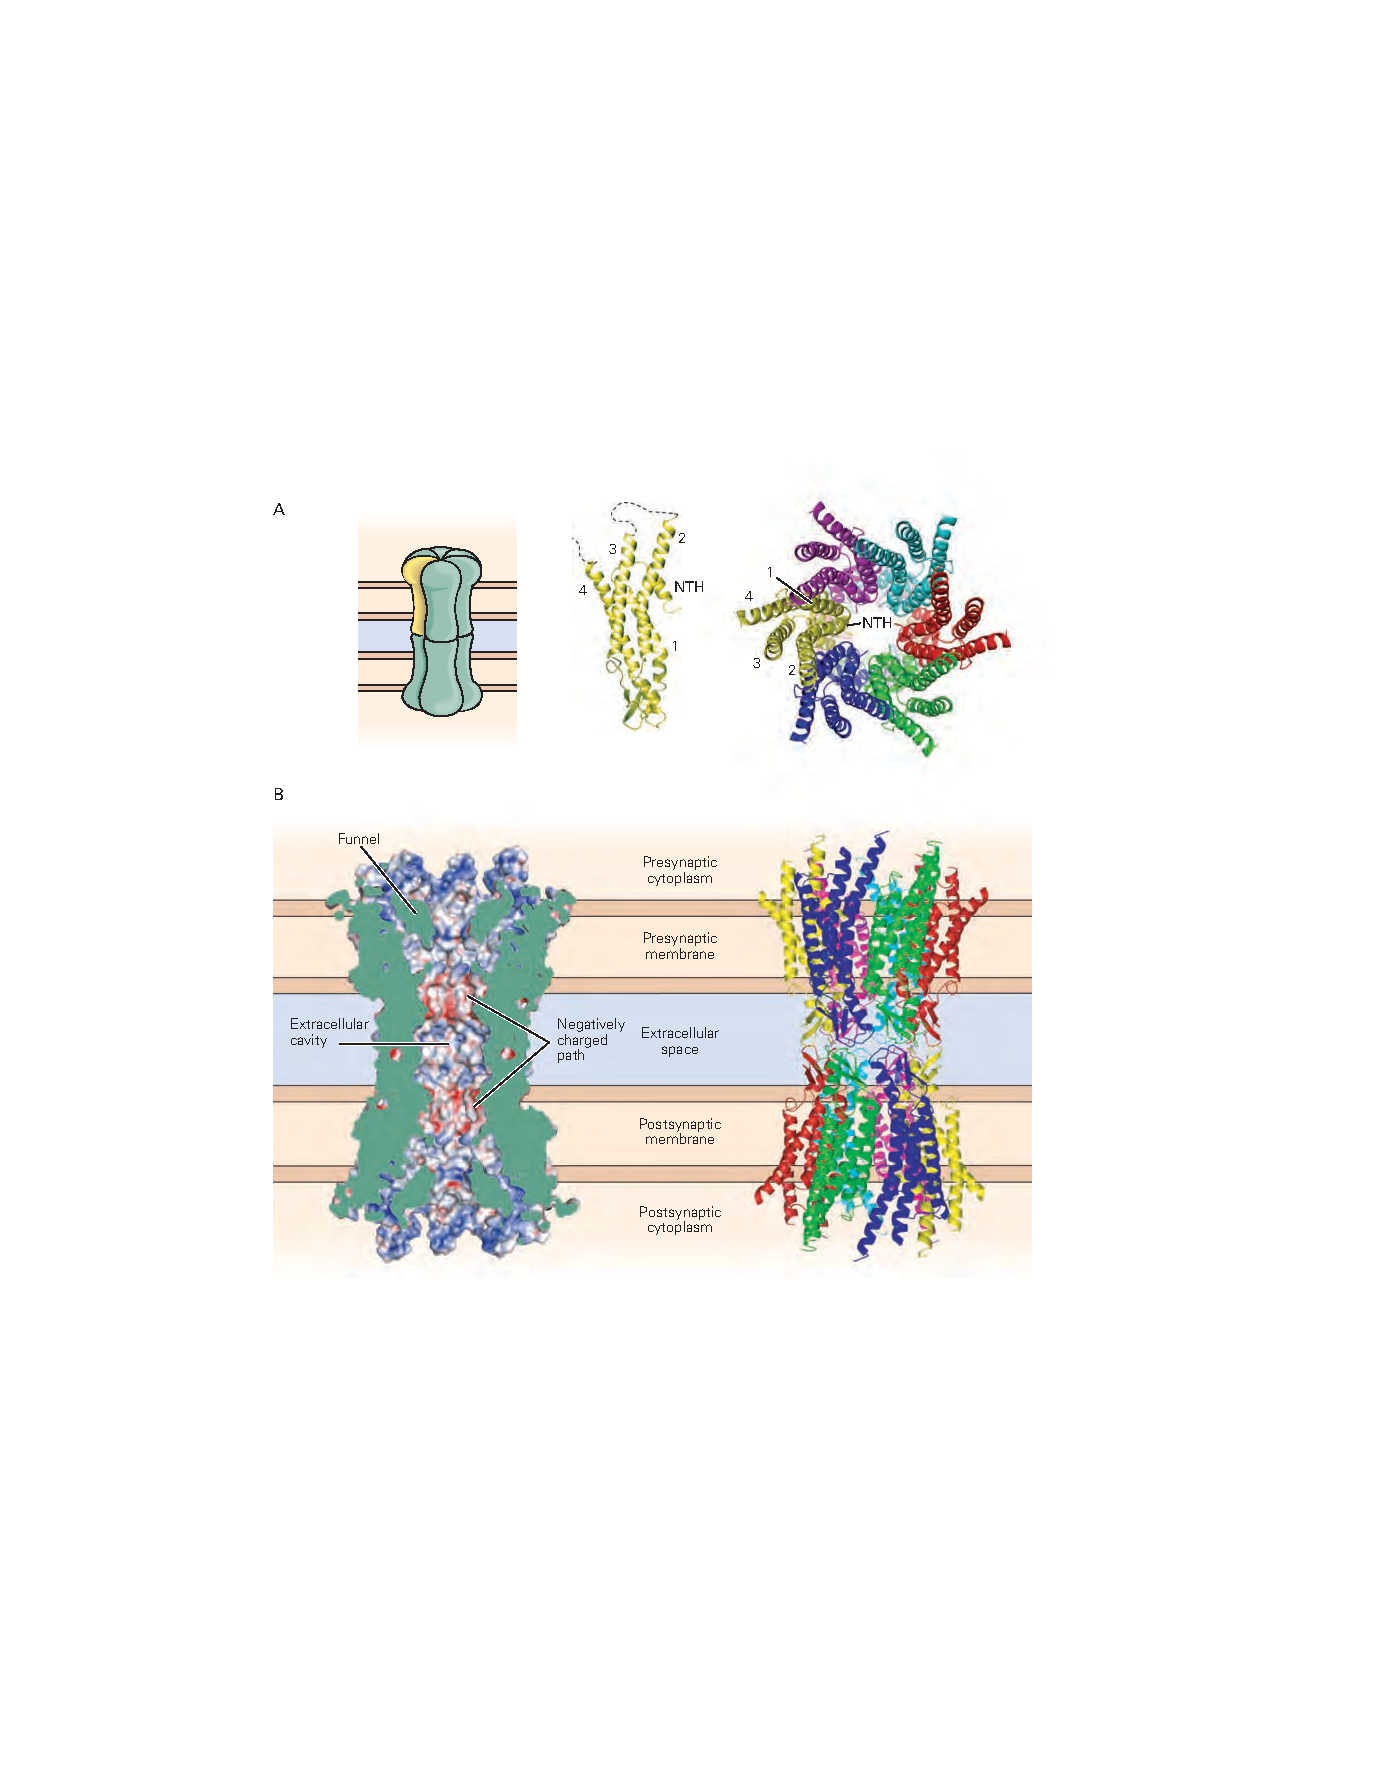
\includegraphics[width=0.9\linewidth]{chap11/fig_11_5}
	\caption{\textit{间隙连接通道}的高分辨率三维结构。
		所有结构均由人连接蛋白 26 亚基形成的间隙连接通道的 X 射线晶体学确定。
		\textbf{A.} 左图:完整的间隙连接通道图,显示了一对并列的半通道。
		中图:单个连接蛋白亚基的高分辨率结构显示四个跨膜 $\alpha$ 螺旋(1–4)和一个短的 N 末端螺旋(NTH)。
		亚基的方向对应于右图中黄色亚基的方向。
		右图:从细胞质观察半通道的自下而上视图。
		六个亚基中的每一个都有不同的颜色。
		黄色亚基的螺旋被编号。
		方向对应于左图中黄色半通道的方向,向观察者旋转 90 度。
		\textbf{B.} 膜平面中间隙连接通道的两个侧视图显示两个并列的半通道。
		方向与 A 部分相同。
		左:通过通道的横截面显示通道孔的内表面。
		蓝色表示带正电的表面;
		红色表示带负电的表面。
		细胞质入口(漏斗)孔内的绿色物质被认为代表由 N 端螺旋形成的通道门。
		右图:通道的侧视图以与 A 部分相同的配色方案显示了六个连接蛋白亚基中的每一个。
		整个间隙连接通道大约 9 纳米宽 x 15 纳米高。}
	\label{fig:11_5}
\end{figure}


\subsection{电传输允许互连细胞的快速同步激活}

电突触有何用处?
正如我们所见,电突触传递是快速的,因为它是由细胞之间电流的直接通过引起的。
速度对于逃避反应很重要。
例如,金鱼的甩尾反应是由脑干中的一个巨大神经元(称为\textit{毛特讷氏细胞})介导的,该神经元在电突触处接收感觉输入。
这些电突触使\textit{毛特讷氏细胞}迅速去极化,进而激活尾巴的运动神经元,从而快速逃离危险。


电传输对于协调神经元组的动作也很有用。
因为电流同时穿过所有电耦合细胞的膜,所以几个小细胞可以一起作为一个大细胞。
此外,由于细胞之间的电耦合,网络的有效电阻小于单个细胞的电阻。
因此,根据欧姆定律,激发电耦合细胞所需的突触电流大于激发单个细胞所需的突触电流。
也就是说,电耦合细胞具有更高的点火阈值。
然而,一旦超过这个高阈值,电耦合细胞就会同步放电,因为在一个细胞中产生的电压激活的 \ce{Na+} 电流会非常迅速地传导到其他细胞。


因此,由一组电耦合细胞控制的行为具有重要的适应性优势:它被爆炸性地触发。
例如,当受到严重干扰时,\textit{海兔}会释放出大量的紫色墨水云,提供保护屏。
这种刻板行为是由支配墨腺的三个电耦合运动细胞介导的。
一旦超过这些细胞的动作电位阈值,它们就会同步放电(图~\ref{fig:11_6})。
在某些鱼类中,快速的眼球运动(称为扫视)也由电耦合运动神经元共同激发所介导。
间隙连接在哺乳动物大脑中也很重要,其中电耦合抑制性中间神经元的同步放电会在大量细胞中产生同步的 40 至 100 赫兹(伽马)振荡。


\begin{figure}[htbp]
	\centering
	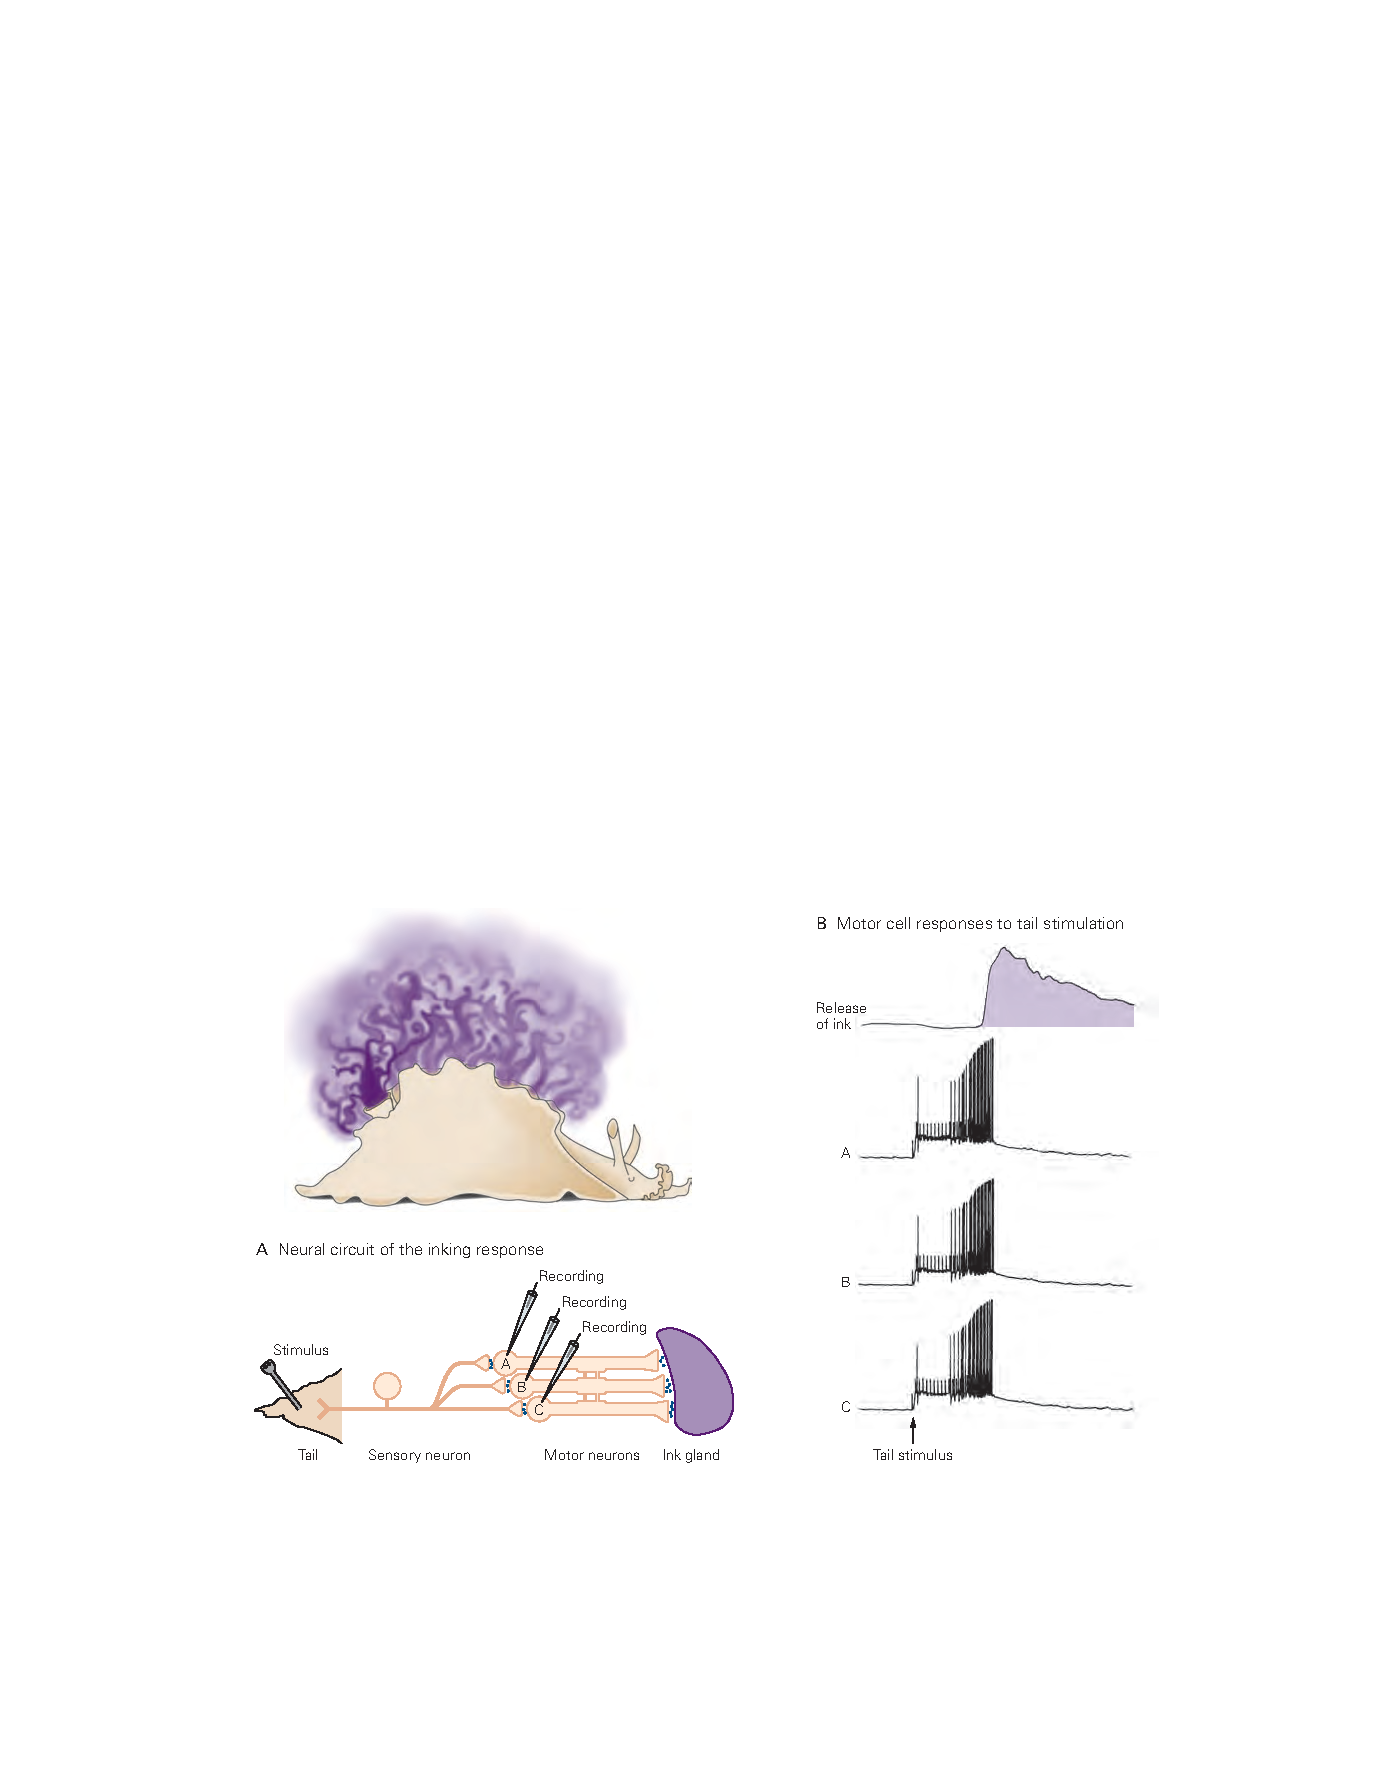
\includegraphics[width=1.0\linewidth]{chap11/fig_11_6}
	\caption{一起放电的电耦合运动神经元可以产生同步行为\cite{carew1976two}。 
		\textbf{A.} 在海螺海兔中,来自\textit{尾部}神经节的感觉神经元与支配\textit{墨腺}的三个\textit{运动神经元}形成突触。
		运动神经元通过电突触相互连接。
		\textbf{B.} 应用于尾巴的一系列刺激会在所有三个运动神经元中产生同步放电,从而导致墨水释放。}
	\label{fig:11_6}
\end{figure}


除了在神经元信号中提供速度或同步性之外,电突触还可以在细胞之间传递代谢信号。
由于其大孔径,间隙连接通道可传导多种无机阳离子和阴离子,包括第二信使钙离子,甚至可传导中等大小的有机化合物(<1 kDa 分子量),如第二信使肌醇 1,4、 5-三磷酸(IP$_3$)、\textit{环磷酸腺苷},甚至小肽。



\subsection{间隙连接在胶质细胞功能和疾病中发挥作用}

间隙连接在胶质细胞之间以及神经元之间形成。
在胶质细胞中,间隙连接介导细胞间和细胞内信号传导。 
在大脑中,单个星形胶质细胞通过间隙连接相互连接,形成神经胶质细胞网络。
脑切片中神经元通路的电刺激可以释放神经递质,从而触发某些星形胶质细胞中细胞内钙离子的升高。
这会产生以大约 1-20 微米每秒的速度从星形胶质细胞传播到星形胶质细胞的钙离子波,比动作电位(10-100 米每秒的传播)慢大约一百万倍。
尽管波的确切功能尚不清楚,但它们的存在表明胶质细胞可能在大脑的细胞间信号传导中发挥积极作用。


间隙连接通道还可以增强某些神经胶质细胞内的交流,例如在周围神经系统中产生轴突髓鞘的雪旺细胞。
由单个雪旺细胞形成的连续髓鞘层通过间隙连接连接。
这些间隙连接可能有助于将髓磷脂层保持在一起,并促进小代谢物和离子穿过多层髓磷脂。
雪旺细胞间隙连接通道的重要性在某些遗传疾病中得到强调。
例如,X 染色体连锁形式的\textit{遗传性神经性肌萎缩}是一种脱髓鞘疾病,是由破坏连接蛋白 32 功能的单一突变引起的,连接蛋白 32 是雪旺细胞中表达的基因。
遗传性突变会阻止耳蜗中连接蛋白(连接蛋白 26)的功能,该连接蛋白通常形成对内耳液体分泌很重要的间隙连接通道,占所有先天性耳聋病例的一半。



\section{化学突触可以放大信号}

与电突触相反,在化学突触中,突触前神经元和突触后神经元之间没有结构连续性。
事实上,化学突触(突触间隙)处两个细胞之间的间隔通常比非突触细胞间隙(20 纳米)稍宽(20-40 纳米)。
化学突触传递依赖于神经递质,神经递质是一种化学物质,可扩散穿过突触间隙并结合并激活靶细胞膜中的受体。
在大多数化学突触中,递质从突触前轴突的特殊肿胀中(突触小球)释放出来,通常包含 100 到 200 个突触小泡,每个小泡都充满了数千个神经递质分子(图~\ref{fig:11_7})。


\begin{figure}[htbp]
	\centering
	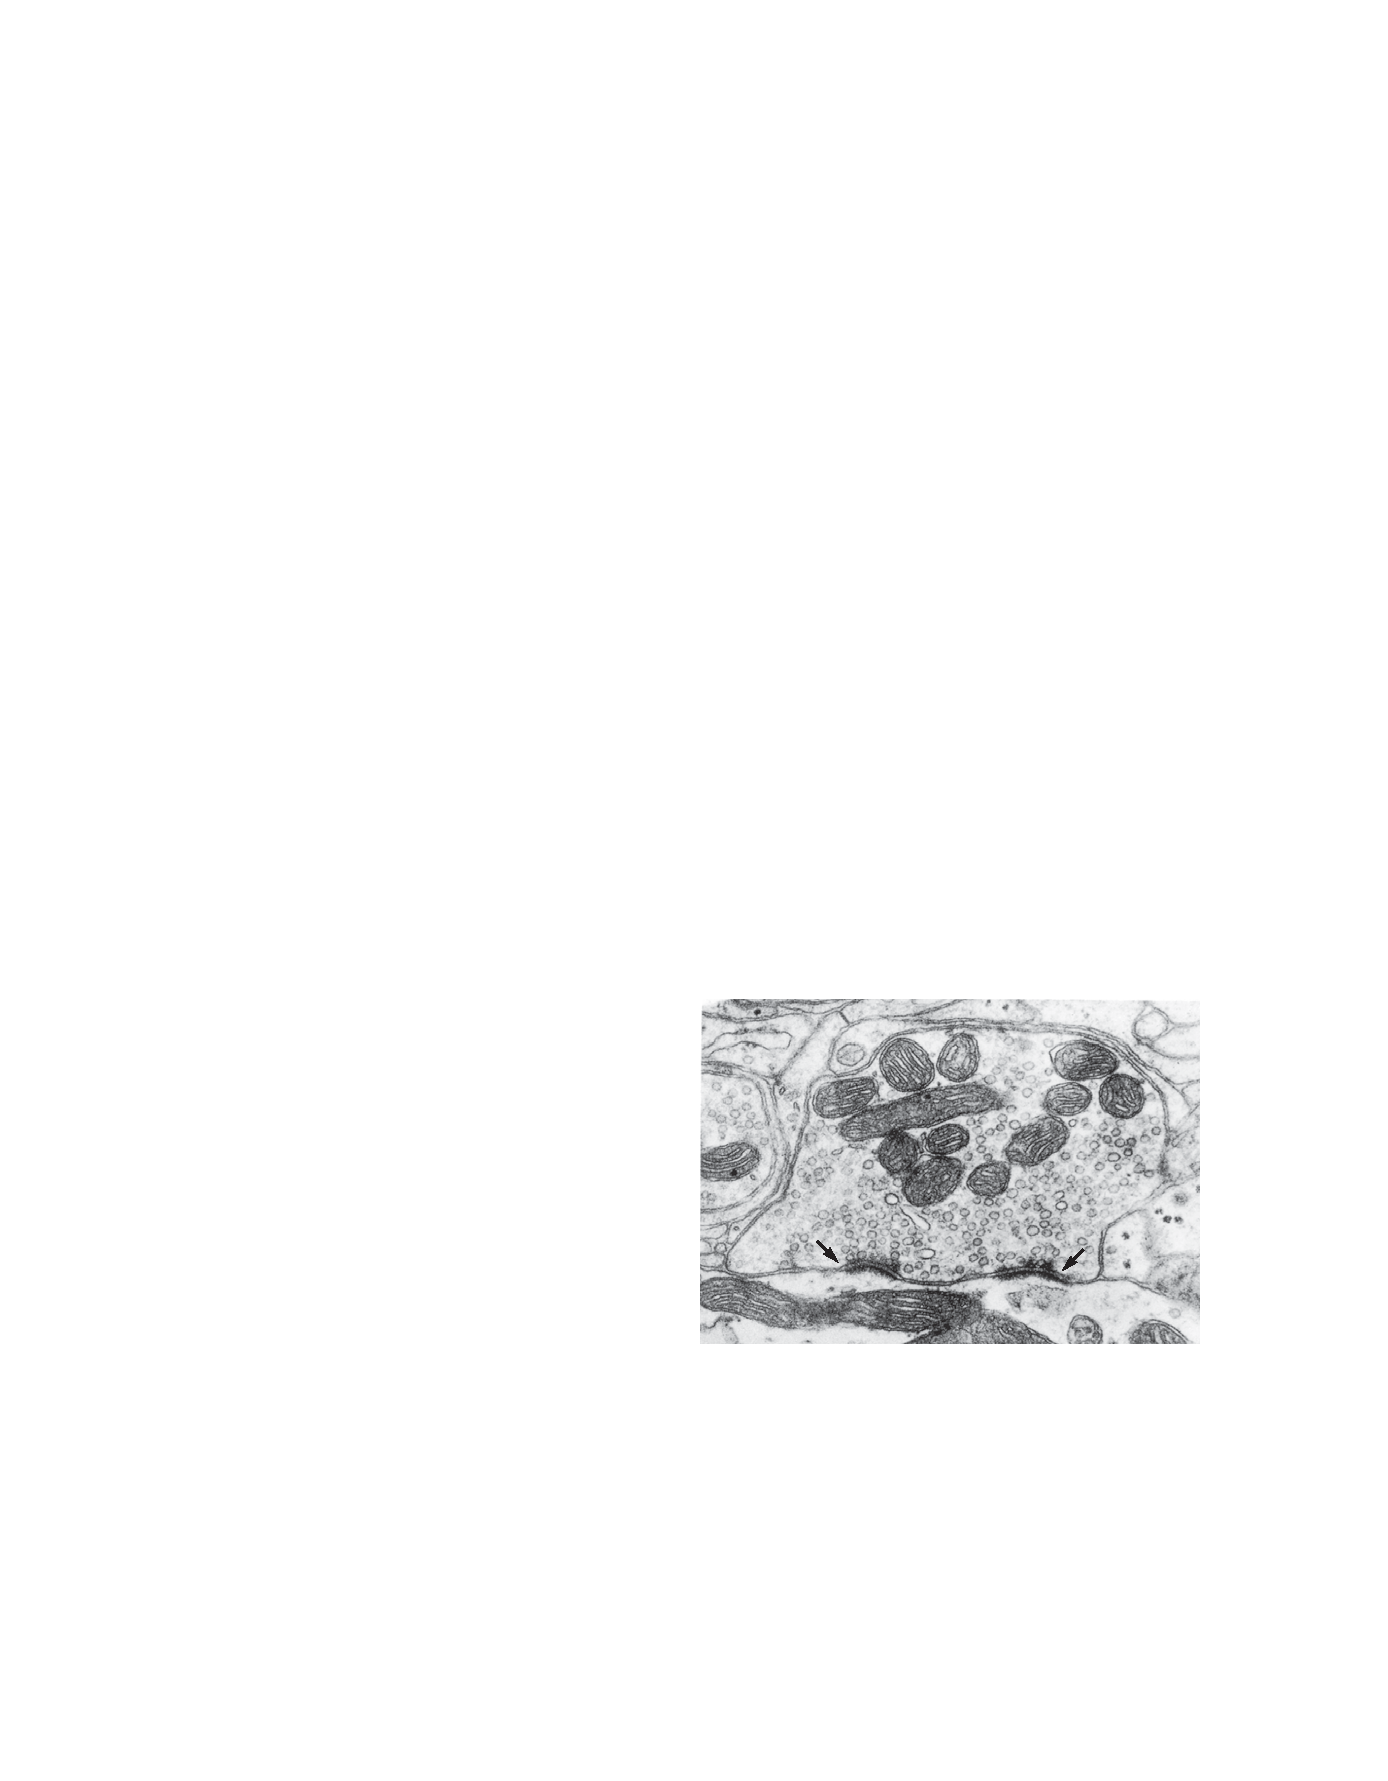
\includegraphics[width=0.55\linewidth]{chap11/fig_11_7}
	\caption{突触前末梢的精细结构。
		这张电子显微照片显示了小脑中的轴突末端。
		大的深色结构是线粒体。
		许多小圆体是含有神经递质的囊泡。
		沿着突触前膜(箭头)的模糊的深色增厚是活动区,被认为是突触小泡停靠和释放位点的专门区域。
		突触间隙是分隔突触前和突触后细胞膜的空间。}
	\label{fig:11_7}
\end{figure}


突触小泡聚集在突触小结的特殊区域,称为活动区。
在突触前动作电位期间,活动区的电压门控钙离子通道打开,允许钙离子进入突触前末梢。
细胞内钙离子浓度的升高会引发生化反应,导致囊泡与突触前膜融合并将神经递质释放到突触间隙中,这一过程称为胞吐作用。
然后,递质分子扩散穿过突触间隙并与突触后细胞膜上的受体结合。
这反过来会激活受体,导致离子通道的打开或关闭。
由此产生的离子通量改变了突触后细胞的膜电导和电位(图~\ref{fig:11_8})。


这几个步骤解释了化学突触的突触延迟。
尽管其生化复杂,但释放过程非常有效,突触延迟通常只有 1 毫秒或更短。
虽然化学传递缺乏电突触的即时性,但它具有重要的放大特性。
仅一个突触小泡就会释放出数千个递质分子,这些递质分子一起可以打开目标细胞中的数千个离子通道。
通过这种方式,仅产生微弱电流的小型突触前神经末梢可以使大型突触后细胞去极化。



\subsection{神经递质的作用取决于突触后受体的特性}

化学突触传递可分为两个步骤:传递步骤,即突触前细胞释放化学信使;
接受步骤,递质结合并激活突触后细胞中的受体分子。
神经元中的传递过程类似于内分泌激素的释放。
事实上,化学突触传递可以被视为激素分泌的一种改良形式。
内分泌腺和突触前末梢都释放具有信号功能的化学物质,两者都是调节分泌的例子(第~\ref{chap:chap7}~章)。
同样,内分泌腺和神经元通常都与其目标细胞有一定距离。


然而,内分泌信号和突触信号之间有一个重要的区别。
腺体释放的激素通过血流传播,直到它与包含适当受体的所有细胞相互作用,而神经元通常只与它形成突触的细胞进行交流。
由于突触前动作电位会触发化学递质释放到距离仅为 20 纳米的目标细胞上,因此化学信号仅传播一小段距离即可到达其目标。 
因此,神经元信号有两个特点:速度快,方向精确。


在大多数神经元中,这种定向或集中释放是在突触神经元的活跃区域完成的。
在没有活动区的突触前神经元神经元中,神经元和激素传递之间的区别变得模糊。
例如,支配平滑肌的自主神经系统中的神经元与它们的突触后细胞有一定距离,并且在它们的末端没有专门的释放位点。
这些细胞之间的突触传递速度较慢,并且依赖于更广泛的递质扩散。
此外,相同的递质物质可以从不同的细胞中以不同的方式释放。
一种物质可以从一个细胞中释放出来,作为直接作用于相邻细胞的传统递质。
从其他细胞中,它可以作为调节剂以不太集中的方式释放,产生更扩散的作用;
从其他细胞中,它可以作为神经激素释放到血液中。


尽管有多种化学物质用作神经递质,包括小分子和肽(第~\ref{chap:chap16}~章),但递质的作用取决于识别和结合递质的突触后受体的特性,而不是递质的化学特性。
例如,\textit{乙酰胆碱}可以激发一些突触后细胞并抑制其他细胞,而在其他细胞中,它可以同时产生兴奋和抑制。
受体决定\textit{乙酰胆碱}的作用,包括胆碱能突触是兴奋性的还是抑制性的。


在一组密切相关的动物中,一种递质物质与保守的受体家族结合,并且通常与特定的生理功能相关。
在脊椎动物中,\textit{乙酰胆碱}作用于所有神经肌肉接头处的兴奋性\textit{乙酰胆碱}受体以触发收缩,同时还作用于抑制性\textit{乙酰胆碱}受体以减慢心率。


传输过程和接收过程之间的区别不是绝对的;
许多突触前终端包含可以修改释放过程的递质受体。
在某些情况下,这些突触前受体被从同一突触前末端释放的递质激活。
在其他情况下,突触前末梢可以与释放不同神经递质的其他神经元类别的突触前末梢联系。


受体的概念在 19 世纪末由德国细菌学家\textit{保罗$\cdot$埃尔利希}引入,用于解释毒素和其他药理学试剂的选择性作用以及免疫反应的高度特异性。
1900 年,\textit{埃尔利希}道:“化学物质只能对能够与之建立密切化学关系的组织元素发挥作用……[这种关系] 必须是特定的。
[化学]基团必须相互适应……就像锁和钥匙一样。”


1906年,英国药理学家约翰兰利假设骨骼肌对箭毒和尼古丁的敏感性是由“接受分子”引起的。
受体功能理论后来由\textit{兰利}的学生(特别是\textit{希勒}和\textit{亨利$\cdot$戴尔})发展,该发展基于同时研究酶动力学和小分子与蛋白质之间的协同相互作用。
正如我们将在下一章中看到的那样,兰利的“接受分子”已被分离出来,并被定性为神经肌肉接头的\textit{乙酰胆碱}受体。


所有化学递质受体都有两个共同的生化特征:

1. 它们是跨膜蛋白。
暴露于细胞外部环境的区域识别并结合来自突触前细胞的递质。


2. 它们在靶细胞内执行效应器功能。
受体通常影响离子通道的打开或关闭。



\subsection{突触后受体的激活直接或间接地控制离子通道}

神经递质直接或间接控制突触后细胞离子通道的开放。
这两类递质作用是由来自不同基因家族的受体蛋白介导的。


直接控制离子通道的受体,例如神经肌肉接头处的\textit{乙酰胆碱}受体,由四个或五个亚基组成,形成一个大分子。
此类受体既包含形成递质结合位点的细胞外结构域,又包含形成离子传导孔的跨膜结构域(图~\ref{fig:11_9}A)。
这种受体通常被称为离子型受体,因为该受体直接控制离子通量。
结合神经递质后,受体会发生构象变化,从而打开离子通道。
第~\ref{chap:chap12}~章和第~\ref{chap:chap13}~章详细讨论了离子型受体(也称为受体通道或配体门控通道)的作用。


\begin{figure}[htbp]
	\centering
	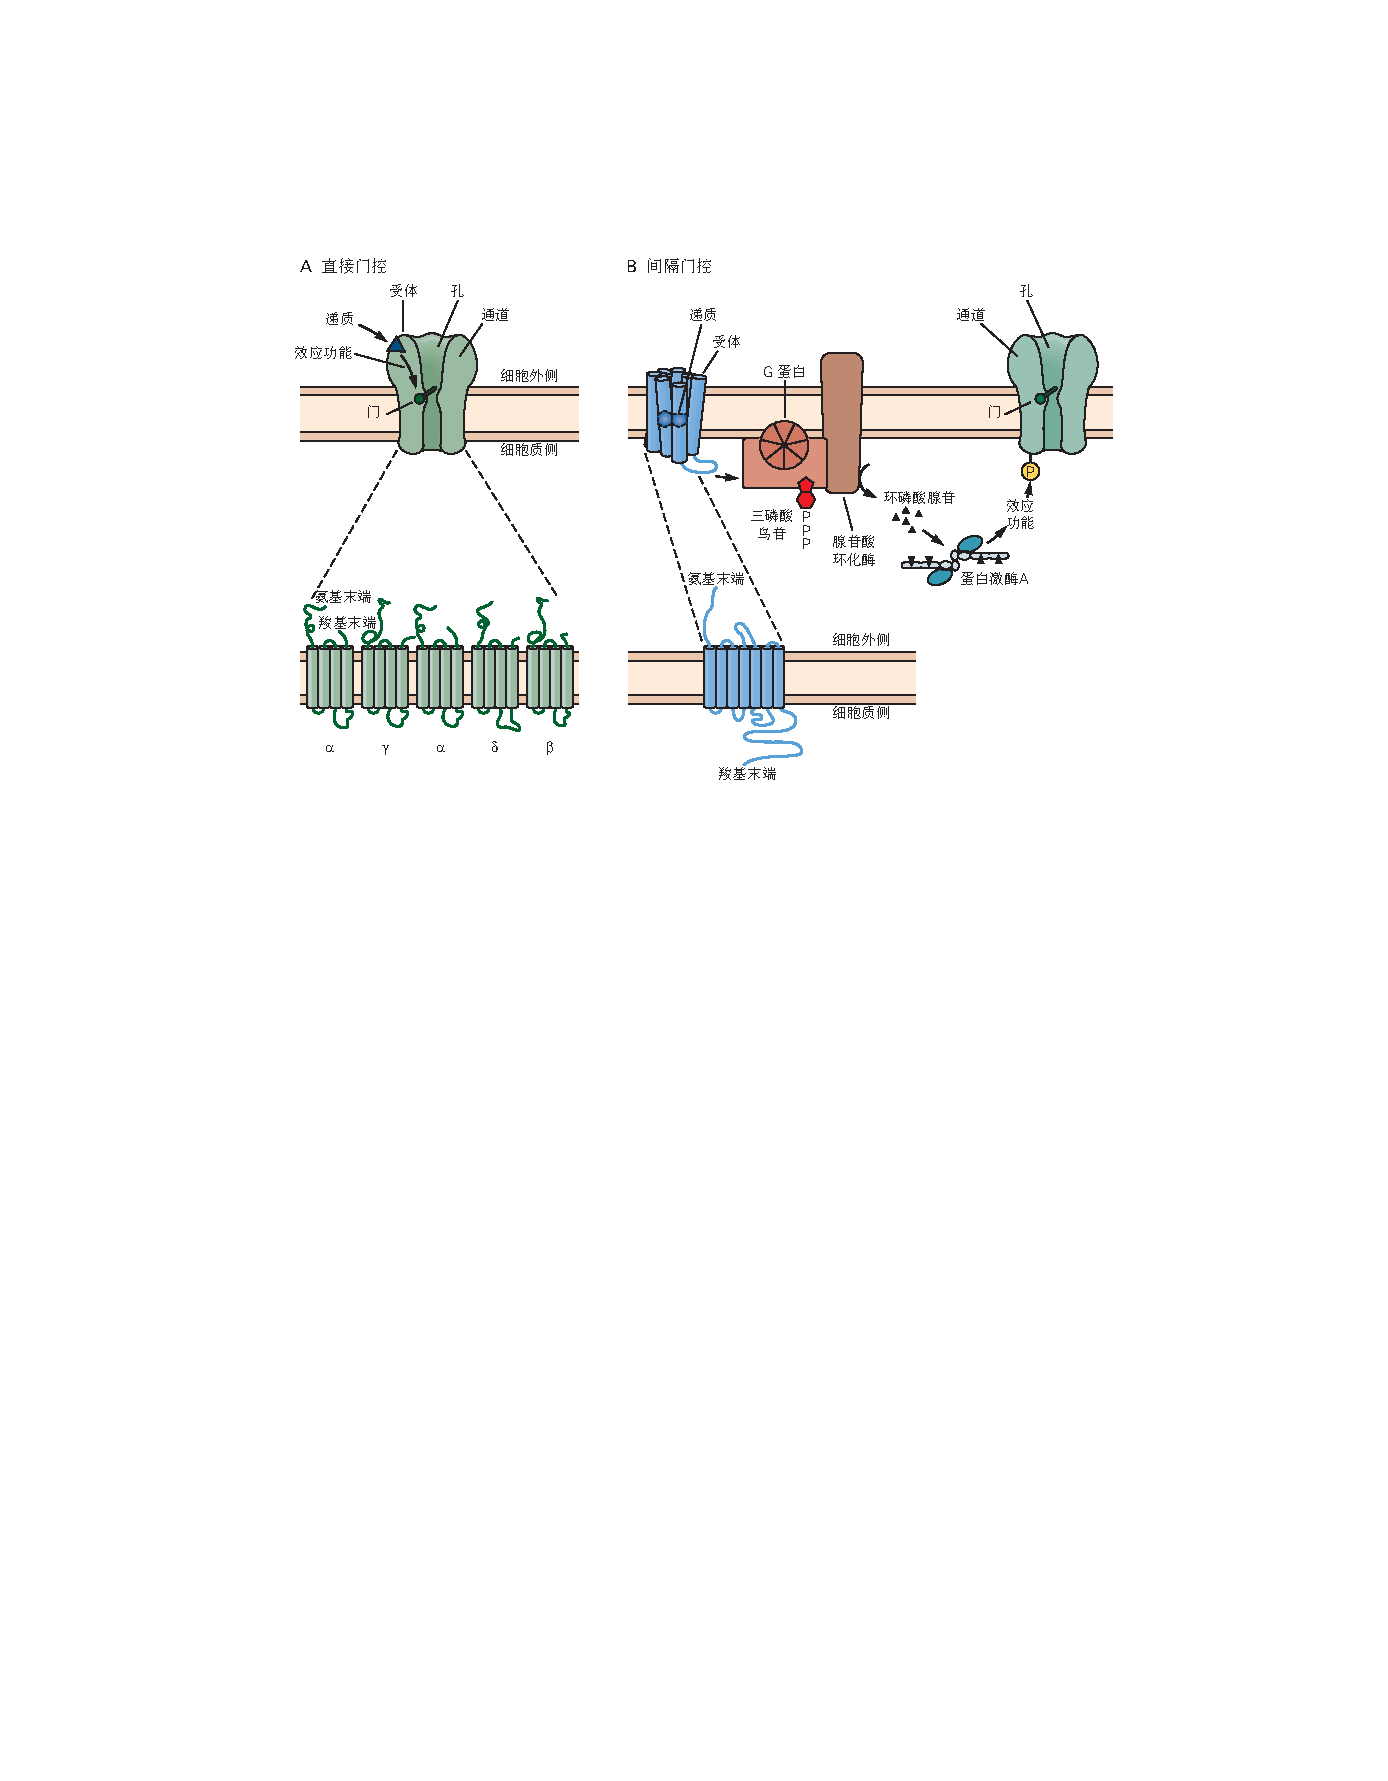
\includegraphics[width=0.87\linewidth]{chap11/fig_11_9}
	\caption{神经递质直接或间接打开突触后离子通道。
		\textbf{A.} 直接打开离子通道的受体是形成通道的大分子的组成部分。 许多此类配体门控通道由五个亚基组成,每个亚基被认为包含四个跨膜 $\alpha$ 螺旋区域。
		\textbf{B.} 间接打开离子通道的受体是独立于它调节的通道的独特大分子。
		在此类受体的一个大家族中,受体由一个亚基组成,该亚基具有七个跨膜 $\alpha$ 螺旋区域,可在膜平面内结合配体。
		这些受体激活\textit{三磷酸鸟苷结合蛋白},后者又激活调节通道活动的第二信使级联。
		在这里所示的级联中,G 蛋白刺激腺苷酸环化酶,将三磷酸腺苷转化为\textit{环磷酸腺苷}。
		\textit{环磷酸腺苷}激活\textit{环磷酸腺苷}依赖性\textit{蛋白激酶A},后者使通道(P)磷酸化,导致开口发生变化。}
	\label{fig:11_9}
\end{figure}


间接门控离子通道的受体,如大脑皮层神经元中的几种去甲肾上腺素或多巴胺受体,通常由一个或至多两个与其调节的离子通道不同的亚基组成。
这些受体通常具有七个跨膜 $\alpha$-螺旋,通过改变细胞内代谢反应发挥作用,通常被称为促代谢受体。
这些受体的激活通常会刺激第二信使的产生,即小的可自由扩散的细胞内代谢物,例如\textit{环磷酸腺苷}或甘油二酯。
许多这些第二信使激活蛋白激酶,磷酸化不同底物蛋白的酶。
在许多情况下,蛋白激酶直接磷酸化离子通道,包括间隙连接通道和离子型受体,调节它们的打开或关闭(图~\ref{fig:11_9}B)。 
第~\ref{chap:chap14}~章详细研究了促代谢受体的作用。


离子型和代谢型受体具有不同的功能。
离子型受体产生仅持续几毫秒的相对快速的突触动作。
这些通常在神经回路的突触中发现,这些突触介导快速行为,例如牵张感受器反射。
促代谢受体产生较慢的突触动作,持续数百毫秒到几分钟。
这些较慢的动作可以通过改变神经元的兴奋性和介导行为的神经回路中突触连接的强度来调节行为。
这种调节性突触动作通常在学习过程中充当重要的强化途径。




\section{电突触和化学突触可以共存并相互作用}

我们现在意识到,\textit{亨利$\cdot$戴尔}和\textit{埃克尔斯}分别对化学突触和电突触的存在都是正确的。
此外,我们现在知道两种形式的突触传递可以共存于同一个神经元中,并且电突触和化学突触可以改变彼此的功效。
例如,在发育过程中,许多神经元最初由电突触连接,电突触的存在有助于化学突触的形成。
随着化学突触开始形成,它们通常会启动电传输的下调。


两种类型的突触也可以共存于成熟神经系统的神经元中。 
这两种突触的作用可能在视网膜回路中得到最好的理解。
在那里,杆状和锥状光感受器释放神经递质谷氨酸,并在一类称为双极细胞的中间神经元上形成化学突触。
每个双极细胞水平延伸其树突,接收来自许多覆盖的视杆细胞和视锥细胞的化学突触输入,这些视杆细胞和视锥细胞对来自视野非常小区域的光作出反应。
然而,双极神经元的感受野大约是它接收化学突触输入的光感受器感受野的两倍。
这是相邻双极细胞之间以及双极细胞与第二种中间神经元(无长突细胞)之间形成电突触的结果(第~\ref{chap:chap22}~章)。


最后,间隙连接的功效可以通过不同蛋白激酶的磷酸化来调节,这通常会增强间隙连接耦合。
例如,多巴胺和其他递质可以通过作用于代谢型 G 蛋白偶联受体来调节\textit{环磷酸腺苷}水平,从而增强或降低通道磷酸化,从而增加或减少间隙连接偶联。
这种复杂的信号循环是许多神经回路的标志,并极大地扩展了它们的计算能力。



\section{亮点}

1. 神经元通过两种主要机制进行交流:
\textit{电}突触传递和\textit{化学}突触传递。


2. 电突触形成于称为间隙连接的紧密并列区域,它为电荷在通信神经元的细胞质之间流动提供了直接途径。
这导致非常快速的突触传递,适用于同步神经元群的活动。 


3. 电突触处的神经元通过间隙连接通道连接,间隙连接通道由一对称为连接子的半通道形成,每个半通道由突触前和突触后细胞贡献。
每个连接子都是一个六聚体,由六个称为连接蛋白的亚基组成。 


4. 在化学突触处,突触前动作电位通过胞吐作用触发突触前细胞释放化学递质。
然后递质分子迅速扩散穿过突触间隙,结合并激活突触后细胞中的递质受体。


5. 虽然比电突触传递慢,但化学传递允许通过释放数万个递质分子和激活突触后细胞中成百上千个受体来放大突触前动作电位。


6. 有两大类传递受体。
离子型受体是配体门控离子通道。
递质与细胞外结合位点的结合会触发构象变化,打开通道孔,产生离子电流,根据受体的不同,激发(去极化)或抑制(超极化)突触后细胞。
离子型受体是快速化学突触传递的基础,可介导神经系统中的快速信号传递。


7. 促代谢受体负责第二大类化学突触作用。
这些受体激活细胞内代谢信号通路,通常会导致第二信使的合成,例如调节蛋白质磷酸化水平的\textit{环磷酸腺苷}。
促代谢受体是缓慢的调节突触动作的基础,这些动作有助于行为状态和唤醒的变化。


